\chapter{Implementación}
Habiendo seleccionado las herramientas, en este capítulo se detallan las distintas etapas de desarrollo e implementación del sistema propuesto.


\section{Preparación del entorno de desarrollo}
En esta sección se describen las herramientas de desarrollo que inicialmente se han configurado para implementar la aplicación.

\subsection{Control de versiones}
Para el control de versiones se ha usa \textbf{Git}, un sistema distribuido que permite llevar un registro de los cambios realizados en el código fuente de un proyecto. Es una herramienta muy potente y versátil que ha ayudado a completar las tareas de desarrollo y documentación de esta aplicación de manera organizada y documentada. Este proyecto se encuentra alojado en \textit{GitHub}, una plataforma de desarrollo colaborativo que utiliza \textit{Git} como sistema de control de versiones; lo que facilitaría la colaboración y el trabajo en equipo si en el futuro alguien decide participar en el desarrollo del proyecto.

\subsection{Entorno de desarrollo integrado (IDE)}
El IDE elegido ha sido \textbf{Visual Studio Code}\footnote{\url{https://code.visualstudio.com/}}(Figura \ref{fig:visual_studio_code}), un editor de código fuente multiplataforma desarrollado por Microsoft que ofrece una amplia gama de funcionalidades. En este proyecto son de especial utilidad algunas como el control integrado de \textit{Git}, la detección de errores en tiempo real (también conocido como \textit{linting}) que notifica los errores de sintaxis y de código antes de la ejecución, o la posibilidad de ejecutar comandos directamente en WSL (Subsistema de Windows para Linux). Esta última funcionalidad ha sido fundamental, ya que permite desarrollar y ejecutar aplicaciones en un entorno Linux virtualizado sin la necesidad de contar con Linux nativo en el sistema, como ocurría en la implementación de este proyecto.

\begin{figure}[ht!]
    \centering
    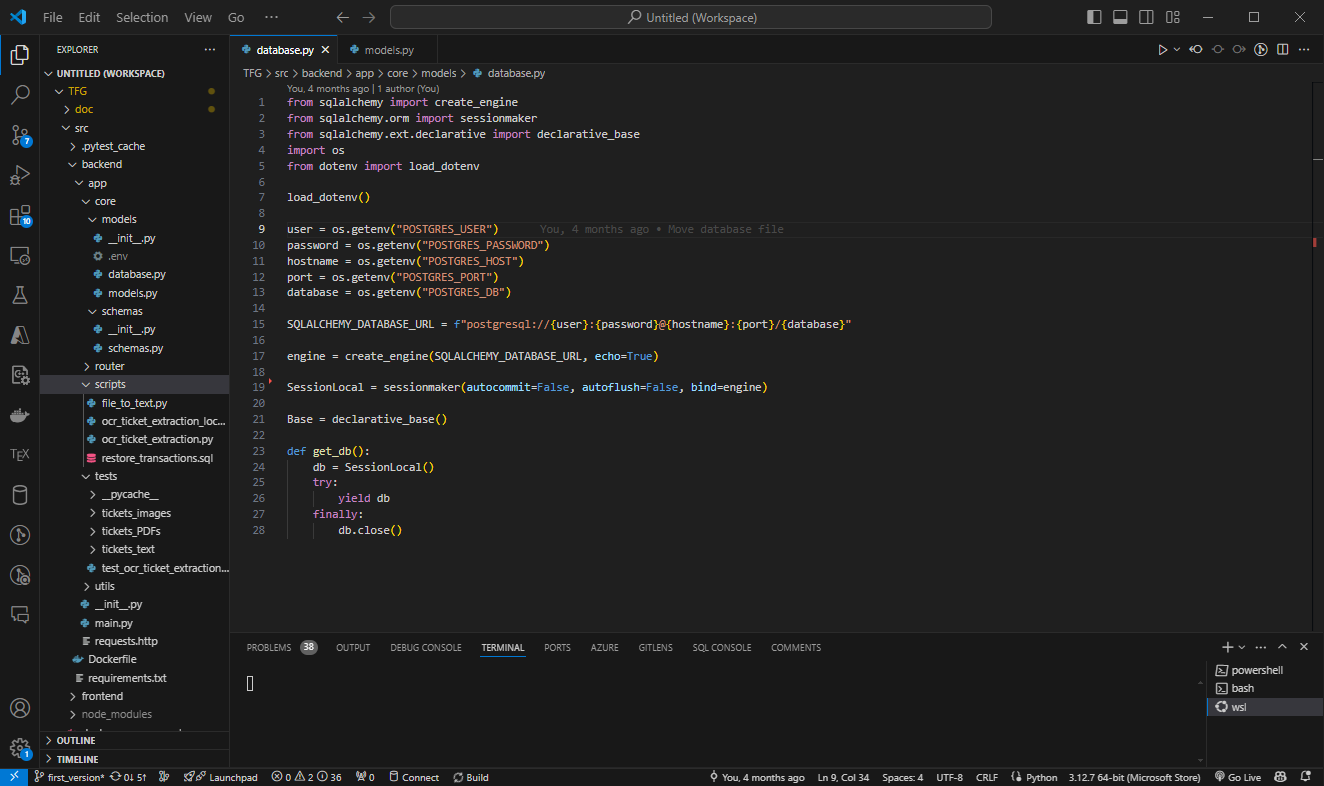
\includegraphics[width=\linewidth]{imagenes/visual_studio_code.png}
    \caption{Visual Studio Code}
    \label{fig:visual_studio_code}
\end{figure}

\subsection{Administrador de base de datos}
Para la gestión de la base de datos se usa \textbf{DBeaver}\footnote{\url{https://dbeaver.io/}}(Figura \ref{fig:dbeaver}), una herramienta de código abierto que permite conectar y administrar bases de datos de diferentes tipos, como MySQL, PostgreSQL, SQLite, Oracle, etc. \textit{DBeaver} dispone de una interfaz gráfica intuitiva que facilita, entre otros, la creación y modificación de tablas, la ejecución de consultas SQL, generación de backups.

\begin{figure}[ht!]
    \centering
    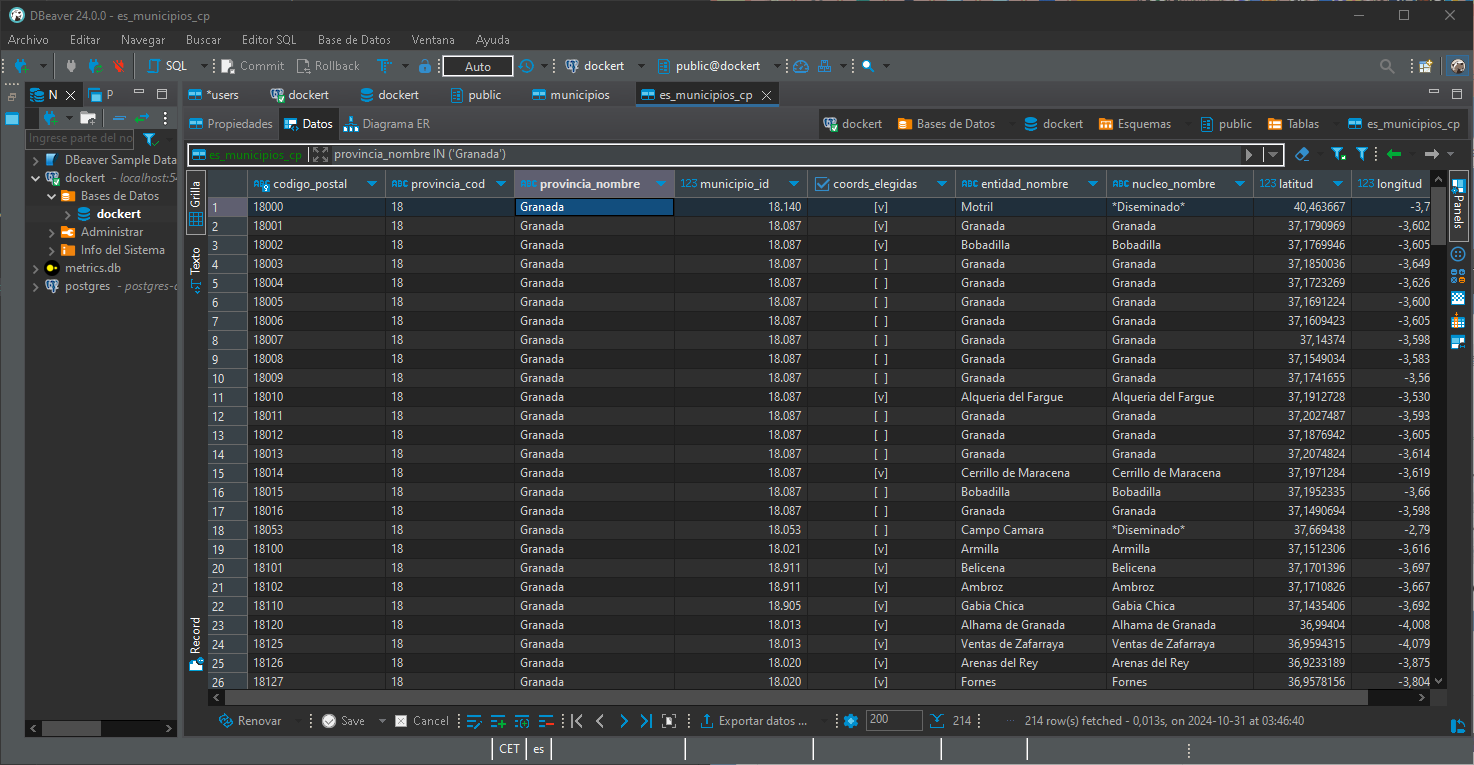
\includegraphics[width=\linewidth]{imagenes/dbeaver.png}
    \caption{Dbeaver}
    \label{fig:dbeaver}
\end{figure}

\subsection{Contenerización}
En el desarrollo de esta aplicación se ha utiliza \textbf{Docker}\footnote{\url{https://www.docker.com/}}(Figura \ref{fig:docker}), una plataforma de código abierto que permite a los desarrolladores empaquetar y distribuir aplicaciones en contenedores. Los contenedores son entornos ligeros y portables que contienen todo lo necesario para ejecutar una aplicación, incluidas las bibliotecas, las dependencias y el código. El uso de \textit{Docker} en este proyecto facilita la creación de entornos de desarrollo y producción consistentes y replicables, lo que garantiza que la aplicación se ejecute de forma similar en cualquier entorno.
\begin{figure}[ht!]
    \centering
    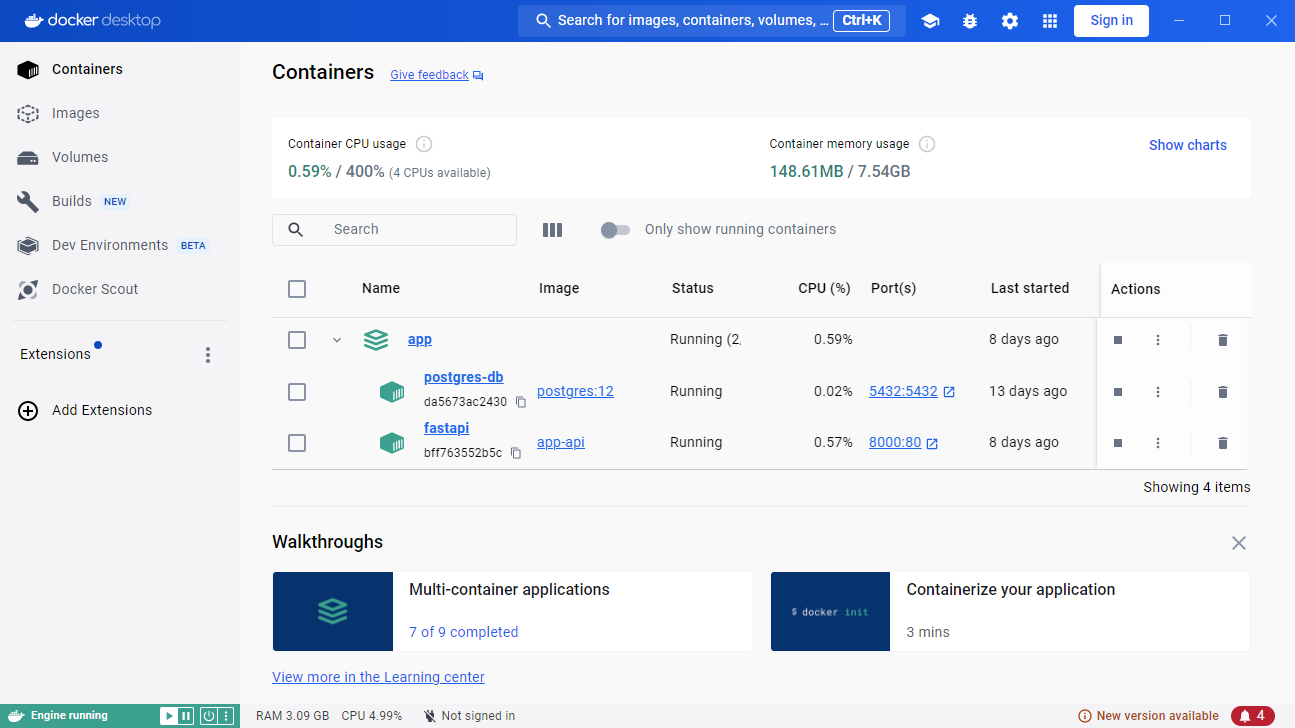
\includegraphics[width=\linewidth]{imagenes/docker.png}
    \caption{Docker}
    \label{fig:docker}
\end{figure}


\section{Creación del backend: Milestone 1}\label{chap:milestone1}
A continuación se describen los pasos seguidos para la implementación del backend de la aplicación utilizando las herramientas seleccionadas.

La implementación se realiza usando Docker, ya que facilita la creación de entornos de desarrollo y producción consistentes, replicables y más seguros, quedando dos servicios interrelacionados: una API desarrollada con FastAPI y una base de datos PostgreSQL; cada uno con una configuración concreta. 

Se crea un contenedor a partir de la imagen oficial de PostgreSQL (versión 12), el sistema de gestión de bases de datos relacional elegido.

FastAPI no se instala a partir de una imagen existente como tal, sino que se crea una personalizada a partir de una imagen ya existente de Python en su versión 3.10, el resto de configuraciones para utilizar FastAPI se extraen del archivo \textit{Dockerfile} creado en los ficheros del backend de la aplicación. Este archivo contiene las instrucciones para instalar las dependencias necesarias y configurar el entorno de ejecución de la aplicación dentro del entorno completo de Python que proporciona la imagen base. 

\begin{itemize}
    \item \textbf{Modelo de la base de datos}\\
        Se crean tablas en la base de datos como clases de Python utilizando SQLAlchemy, lo que permite definir las relaciones entre tablas para garantizar la integridad de los datos y se han definido restricciones para asegurar la coherencia de la información. Las clases se encargan de mapear los objetos de Python a las tablas de la base de datos, facilitando la interacción con la base de datos y la manipulación de los mismos.

El diagrama entidad-relación (Figura \ref{fig:diagrama_ER}) es una representación gráfica de las entidades que permite visualizar el esquema de las tablas en la base de datos.

\begin{figure}[ht!]
    \centering
    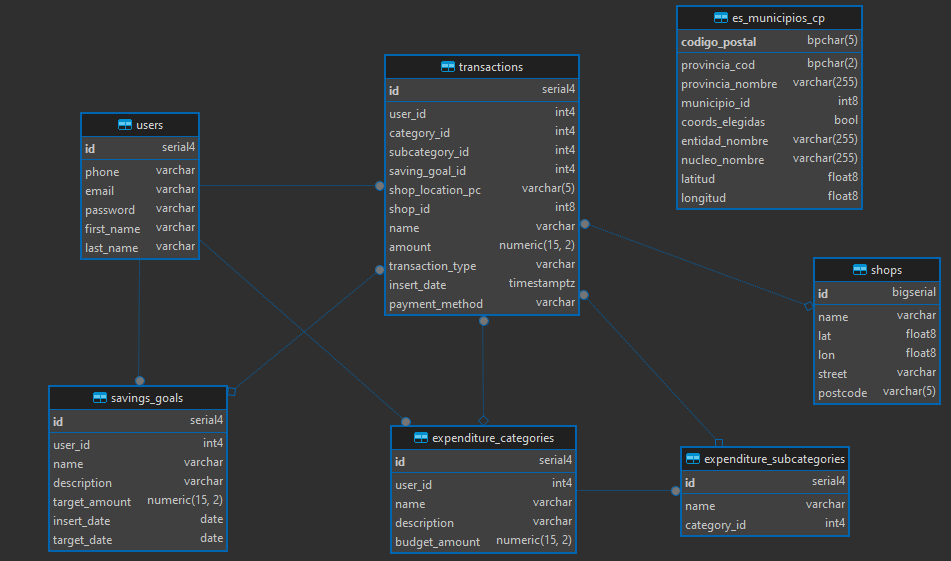
\includegraphics[height=70mm]{imagenes/diagrama_ER.png}
    \caption{Diagrama Entidad-Relación de la capa de datos (en DBeaver).}
    \label{fig:diagrama_ER}
\end{figure}


    \item \textbf{Esquemas de validación}\\
        Aprovechando la integración de FastAPI con Pydantic, se crean esquemas de validación para cada entidad, lo que facilita la validación de los datos en las solicitudes HTTP, aportando seguridad y consistencia a la aplicación.

    \item \textbf{Endpoints}\\
        Se crean los endpoints de la API REST utilizando FastAPI, definiendo las rutas y los métodos HTTP que utilizar para interactuar con la API. Para ello se implementan las operaciones CRUD \textit{(Create, Read, Update, Delete)} para cada entidad de la base de datos, lo que permite realizar las operaciones básicas de gestión de datos.

    \item \textbf{Persistencia}\\
        Con una configuración simple de volúmenes en Docker, se garantiza la persistencia de los datos en la base de datos PostgreSQL. Con la definición del volumen persistente, los datos se almacenan fuera del contenedor, lo que asegura que estos se mantengan incluso después de reiniciar el contenedor o eliminarlo.

    \item \textbf{Pruebas}\\
        Se revisa con DBeaver la correcta creación y estructura de las tablas en la base de datos.
        Desde la documentación generada automáticamente en FastAPI, se realizan varios tipos de pruebas básicas para verificar el funcionamiento correcto de los endpoints y la interacción con la base de datos. Entre ellas se realizan algunas pruebas de conectividad a la base de datos (comprobando que se podía acceder a los datos), pruebas CRUD para examinar las operaciones de creación, lectura, actualización y eliminación de cada entidad y pruebas de validación de datos para comprobar que las restricciones definidas en los esquemas de validación son detectadas correctamente.
\end{itemize}

\subsubsection{Componente backend}
Finalmente, se obtiene un componente backend funcional que proporciona una API REST básica para la gestión de datos de la aplicación. Este componente se encarga de la gestión de la base de datos y la validación de los mismos. Permite la interacción con el frontend cuyo desarrollo se hará en el siguiente milestone. En la Figura \ref{fig:endpoints} se muestran algunos de los endpoints creados, concretamente los relacionados con las operaciones de las entidades que representan a las subcategorías, las transacciones de forma general y más concretamente las transacciones de tipo \textit{ingreso}. La documentación de la API generada automáticamente por FastAPI permite visualizar estos endpoints y realizar las pruebas mencionadas de forma sencilla.

\begin{figure}[ht!]
    \centering
    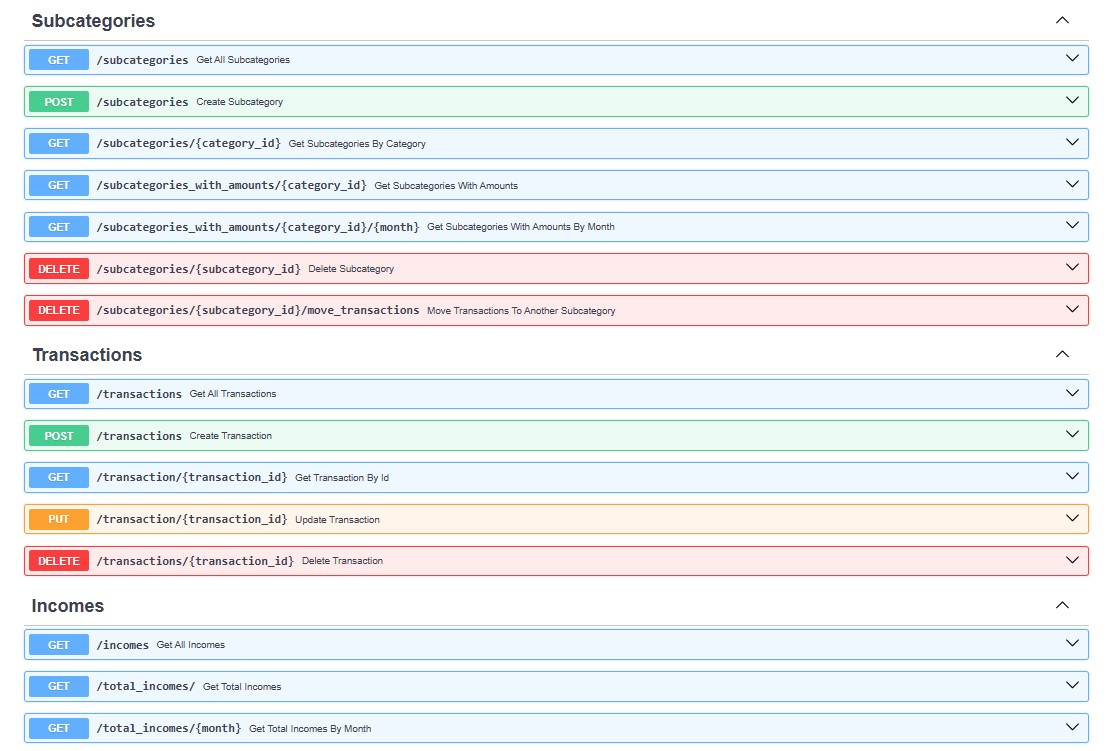
\includegraphics[width=\linewidth]{imagenes/endpoints.jpg}
    \caption{Endpoints de la API REST}
    \label{fig:endpoints}
\end{figure}


\section{Creación del frontend: Milestone 2}\label{chap:milestone2}
La aplicación presenta varias vistas con estructura similar, pero diferente información, por ello se ha priorizado la reutilización de componentes todo lo posible, para facilitar el mantenimiento, la escalabilidad y la coherencia visual.


El diseño de componentes se ayuda de herramientas como \textbf{Tailwind CSS} junto con \textbf{DaisyUI}, que permiten usar componentes preconstruidos y estilos atractivos de forma rápida y sencilla. Y las bibliotecas \textbf{Heroicons} y \textbf{Headless UI}, que ofrecen iconos y componentes fáciles de incorporar.


\begin{itemize}
    \item \textbf{Componentes reutilizables}\\
        Se crean componentes reutilizables para elementos comunes en la aplicación, como botones, formularios, etc. Esto permite mantener la coherencia visual y facilita la creación de nuevas vistas.
    \item \textbf{Rutas}\\
        Se definen las rutas de la aplicación, que permiten al usuario navegar entre las diferentes vistas. Se crean rutas para cada vista y se definen las acciones que se deben realizar al acceder a cada ruta.
    \item \textbf{Interacción con la API}\\
        La forma en que el frontend es capaz de realizar solicitudes es con la biblioteca \textbf{Axios}, que permite realizar solicitudes HTTP de forma sencilla y eficiente. Axios se encarga de enviar las solicitudes al backend con los datos necesarios y de procesar las respuestas, lo que facilita la interacción con la API y la manipulación de los datos. Las solicitudes se generan por la interacción del usuario con la interfaz, por ejemplo, al hacer clic en un botón o al enviar un formulario.
    \item \textbf{Pruebas}\\
        Se han realizado pruebas para verificar el correcto funcionamiento de los componentes y la interacción con la API. Se han comprobado manualmente las rutas, la interacción con los componentes y la visualización de la información en el frontend.
\end{itemize}


\subsection{Operaciones desde la interfaz de usuario}
Se crean los formularios y vistas que servirán al usuario para interactuar con las operaciones implementadas en la API. Entre las operaciones implementadas para que el usuario pueda ejecutarlas en la aplicación web, encontramos:

\begin{itemize}
    \item \textbf{Creación}\\
        El usuario puede crear nuevos elementos, como transacciones, categorías de gasto, objetivos de ahorro, etc. Para ello, la aplicación muestra un formulario con los campos necesarios para la creación del elemento, el usuario debe rellenar los campos y enviar el formulario para que la información se almacene en la base de datos.        
    \item \textbf{Modificación}\\
        Del mismo modo, por medio de un formulario el usuario puede modificar los elementos ya existentes. La aplicación muestra los datos actuales del elemento y permite al usuario modificarlos y guardar los cambios en la base de datos.
    \item \textbf{Eliminación}\\
        La aplicación permite al usuario eliminar todos los elementos que él mismo ha creado. Al hacer clic en el botón de eliminar, la aplicación muestra una confirmación y, si el usuario confirma la eliminación, se elimina el elemento de la base de datos.
    \item \textbf{Visualización de transacciones}\\
        La aplicación muestra al usuario la información de las transacciones almacenadas en la base de datos, permitiendo al usuario ver sus movimientos financieros y analizar su historial.        
\end{itemize}

\subsubsection{Componente frontend}
Finalmente, se obtiene un componente frontend funcional que se encarga de mostrar la información de forma clara y organizada, y permite al usuario interactuar con la aplicación. Los elementos que conforman el frontend permiten al usuario navegar entre las diferentes vistas y realizar las operaciones descritas anteriormente. En la Figura \ref{fig:componentes_frontend} se muestra un esquema de los componentes principales de la aplicación. En las figuras \ref{fig:ingreso_form} y \ref{fig:ingreso_lista} se pueden ver dos elementos del frontend que interactúan con los endpoints de las operaciones de tipo \textit{ingreso} mostradas en el backend.

\begin{figure}[ht!]
    \centering
    \begin{minipage}{0.45\textwidth}
        \centering
        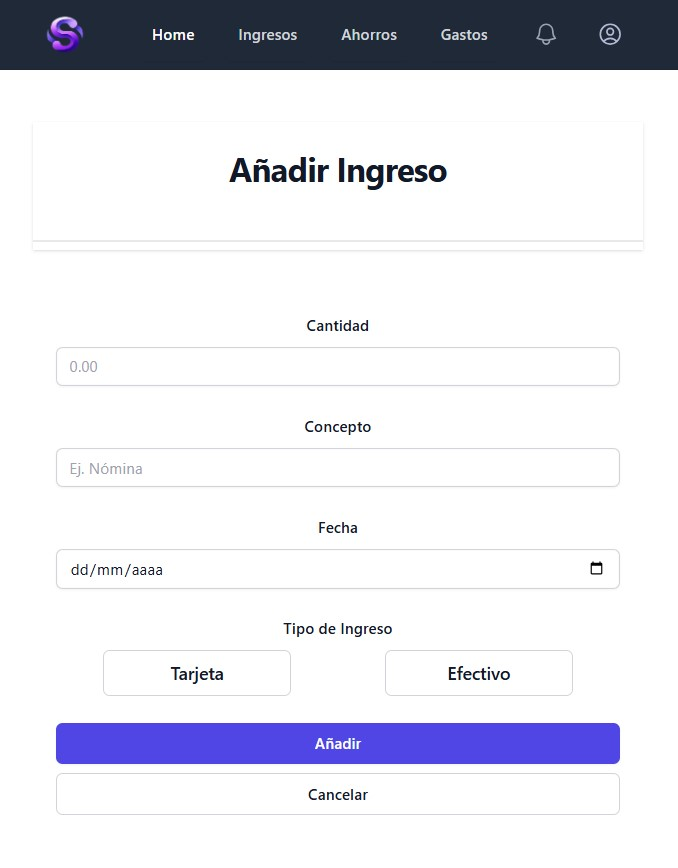
\includegraphics[height = 70mm]{imagenes/ingreso_form.jpg}
        \caption{Elemento frontend para añadir un ingreso}
        \label{fig:ingreso_form}
    \end{minipage}\hfill
    \begin{minipage}{0.45\textwidth}
        \centering
        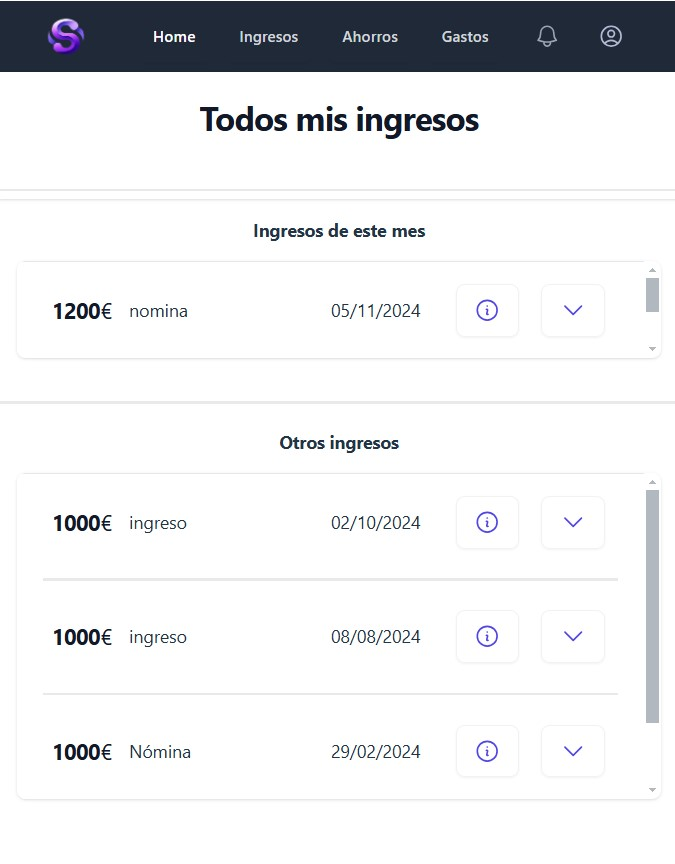
\includegraphics[height = 70mm]{imagenes/ingreso_lista.jpg}
        \caption{Elemento frontend para visualizar la lista de ingresos}
        \label{fig:ingreso_lista}
    \end{minipage}
\end{figure}


\subsubsection{Vistas de la aplicación}
Indagando más en la visualización de transacciones, se han creado diferentes vistas para mostrar la información de las transacciones de forma clara y organizada. Se han creado vistas para mostrar los gastos mensuales por categorías, los ahorros por objetivos, etc. Cada vista muestra la información de forma simple, lo que permite al usuario analizar sus gastos y tomar decisiones informadas sobre su economía.


La navegación entre las diferentes vistas de la aplicación se ha implementado con \textbf{React Router}, para definir rutas y acciones a realizar al acceder a cada una. Se han creado rutas para cada vista, y se ha definido cada vista como un componente de React, con lo que se construye una aplicación de una sola página (SPA, \textit{Single Page Application}) que permite al usuario navegar entre las diferentes vistas sin necesidad de recargar la página en el navegador. 


Entre las diferentes vistas, podemos agruparlas por la funcionalidad de la que se encargan para entender mejor su implementación. Por ejemplo, la modificación o creación de transacciones se hace por medio de formularios, la eliminación suele hacerse con un botón incluido en la visualización del elemento concreto, etc. Cada grupo de vistas está formado por componentes comunes que se reutilizan y por componentes específicos que se encargan de mostrar la información que diferencia una vista de la otra con la que comparte elementos. 


Las principales vistas donde se muestra la información que dará valor a los datos almacenados del usuario se describen a continuación. En la Figura \ref{fig:componentes_frontend} se muestran estas vistas principales y la navegabilidad entre ellas, mostrando su estructura de componentes. Cada caja corresponde a un componente implementado en React.

\begin{itemize}
    \item \textbf{Vista de inicio (\textit{HomeView}).} Muestra por separado la suma total de ingresos, gastos y ahorros del usuario en el mes actual. Se corresponde con el concepto de monedero o cartera, donde el usuario puede ver de un vistazo su situación financiera del mes.
    \item \textbf{Vista de gastos mensuales (\textit{ExpensesOverviewView}).} Muestra la cantidad total de gastos del usuario en el mes actual. Desglosa también la cantidad total entre las diferentes categorías de gasto y mostrando el total acumulado por cada una de ellas y mostrando cuánto queda para llegar al límite del presupuesto establecido.
    \item \textbf{Vista de ahorros (\textit{SavingsOverviewView}).} Muestra la cantidad total apartada como ahorro del usuario en el mes actual. Desglosa también la cantidad total entre los diferentes objetivos de ahorro y muestra el progreso de cada uno de ellos. En este caso, aunque la cifra de resumen total muestra lo ahorrado solo en el mes actual, los objetivos de ahorro se consideran a largo plazo, por lo que se muestra también el total ahorrado hasta el momento para cada uno (incluyendo las aportaciones de meses anteriores).
    \item \textbf{Vista de categoría de gasto (\textit{CategoryView}).} Muestra la cantidad total de gastos del usuario en la categoría seleccionada durante el mes actual, incluyendo los movimientos realizados en cualquier subcategoría perteneciente a la categoría seleccionada.
    \item \textbf{Vista de objetivo de ahorro (\textit{SavingsGoalView}).} Muestra la cantidad total ahorrada por el usuario en el objetivo de ahorro seleccionado durante el mes actual y el total desde que comenzó a ahorrar para dicho objetivo, incluyendo todos los movimientos de ahorro realizados. Muestra también una barra de progreso, que indica cuánto queda para alcanzarlo. 
    \item \textbf{Las vistas de transacciones (\textit{TransactionsView}).} Muestran para el elemento que se consulta todas las transacciones separadas en dos paneles: transacciones del mes actual y transacciones de meses anteriores.
\end{itemize}

\begin{figure}[ht!]
    \centering
    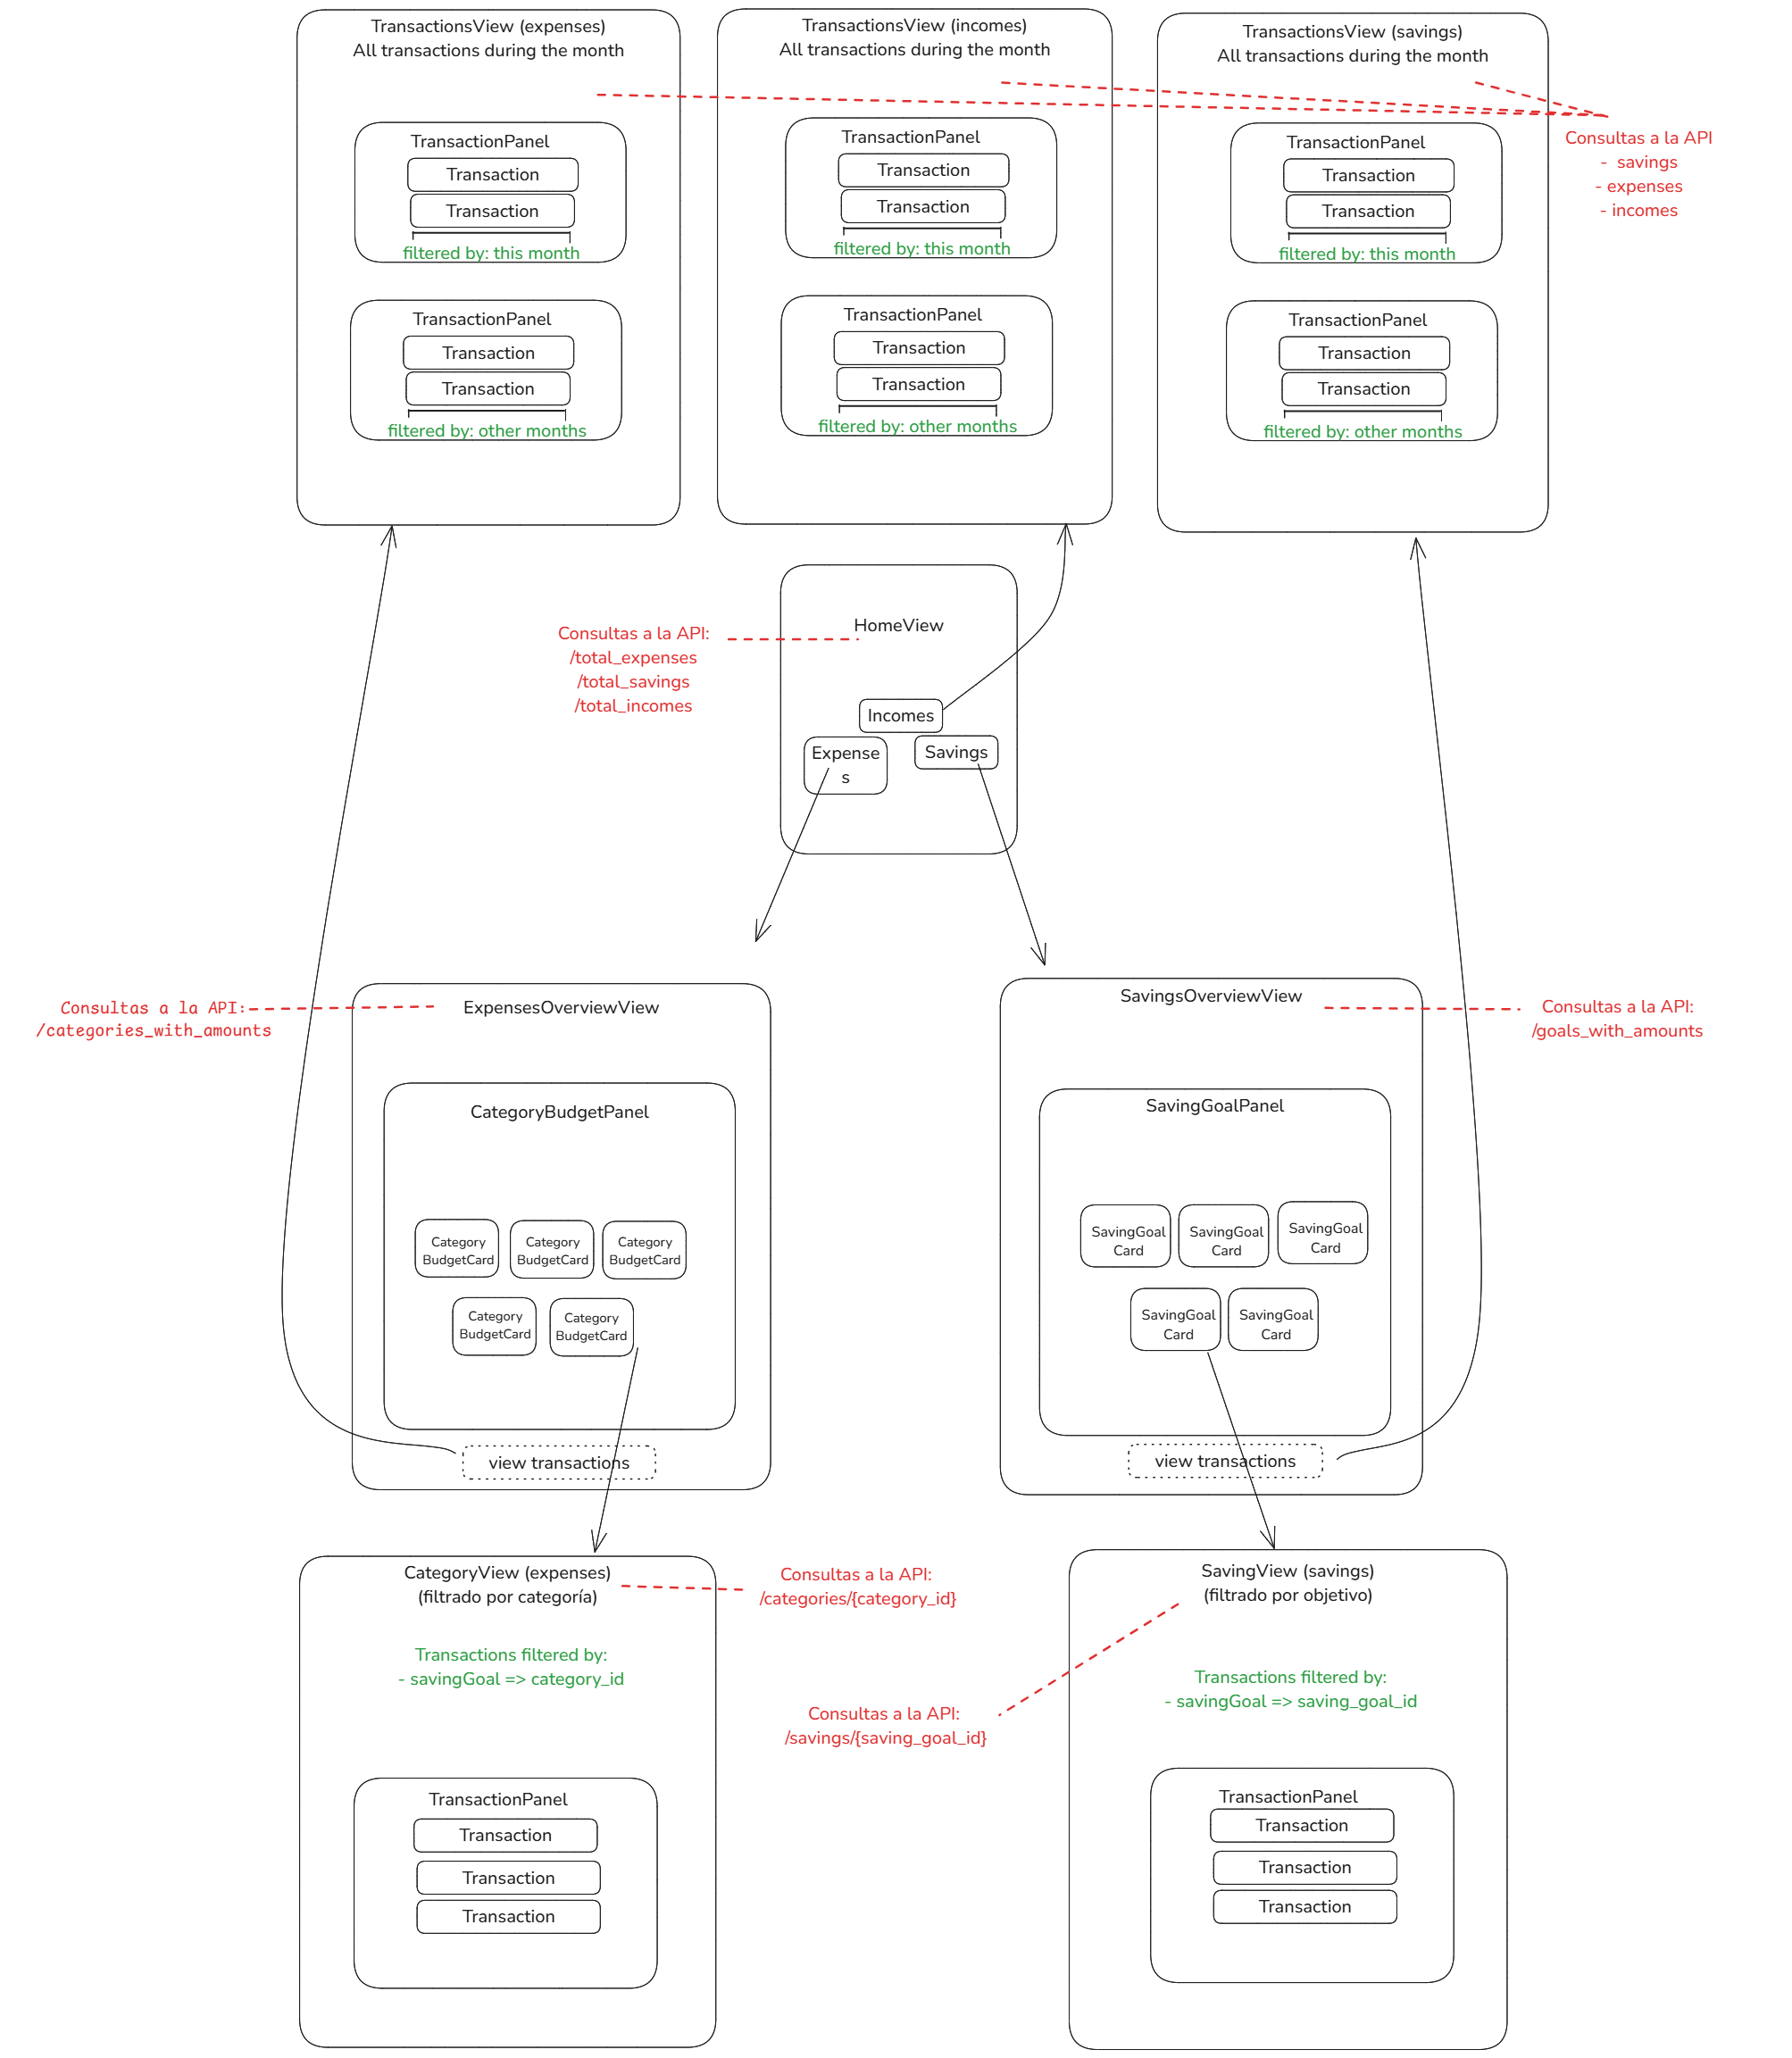
\includegraphics[width=\linewidth]{imagenes/componentes-frontend.png}
    \caption{Vistas principales de la aplicación}
    \label{fig:componentes_frontend}
\end{figure}



\section{Generación de gráficos y resúmenes de transacciones: Milestone 3}\label{chap:milestone3}
En la implementación del frontend, con el fin de facilitar el mantenimiento y la escalabilidad del código, se pueden crear componentes de tipo \textit{smart} y componentes de tipo \textit{dumb}. Los componentes \textit{smart} son aquellos que tienen la lógica de negocio y se encargan de realizar las solicitudes al backend. Por otro lado, los componentes \textit{dumb} son componentes más simples que se encargan de mostrar la información, con los que actúa directamente el usuario. De esta manera, se sigue el principio de responsabilidad única por cada componente. En el desarrollo se ha seguido esta recomendación, aunque no es una regla estricta, por lo que la estructura del código puede variar dependiendo de las necesidades específicas en aplicación o las preferencias del desarrollador\cite{khan2023reactjs}.\\

En este milestone se implementan las funcionalidades de la aplicación que permiten visualizar gráficos y resúmenes de los datos almacenados en la base de datos.

Tomando de ejemplo la vista de ahorros, se describe a continuación cómo se implementa la funcionalidad para incluir gráficos y resúmenes de ahorros en la aplicación. Se refleja claramente la estructura de componentes \textit{smart} y \textit{dumb}, ya que los dos componentes reciben la información desde el componente de vista de ahorros (que es quien realiza la petición con Axios), por lo que se encargan exclusivamente de la representación de la información. En la Figura \ref{fig:componentes_graficos_resumenes} se puede ver qué parte supone cada componente en la vista de ahorros.

\begin{figure}[ht!]
    \centering
    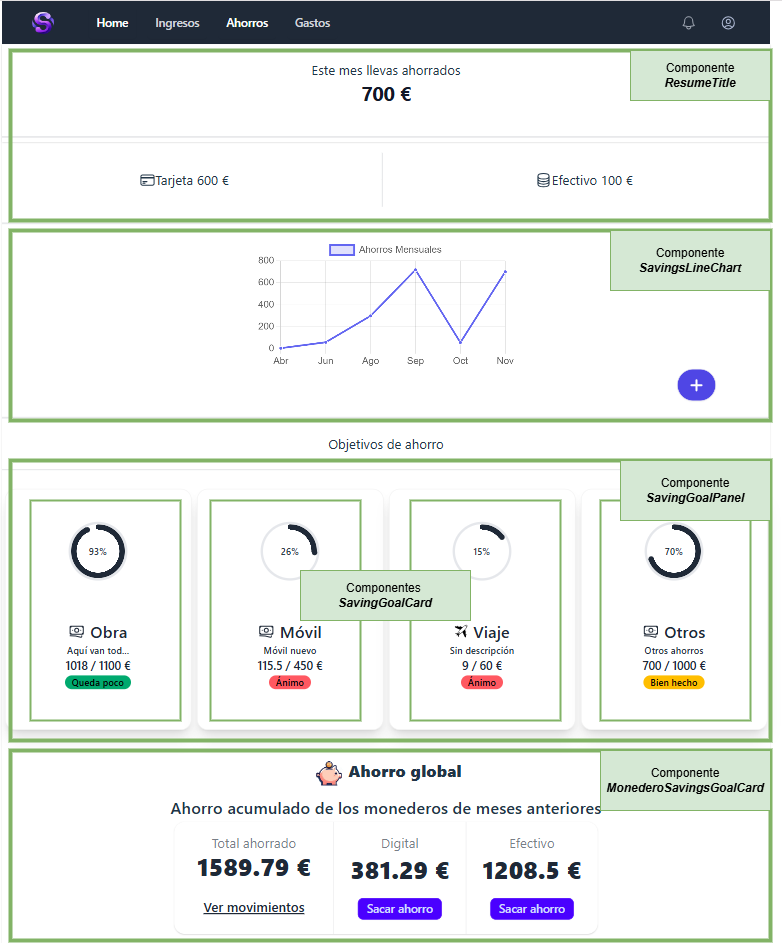
\includegraphics[width=\linewidth]{imagenes/componente-graficos-resumenes.drawio.png}
    \caption{Componentes de gráficos y resúmenes en la vista de ahorros}
    \label{fig:componentes_graficos_resumenes}
\end{figure}


\subsection{Resúmenes}
Los resúmenes creados tienen como objetivo mostrar al usuario de forma clara y concisa la información relevante de los datos del mes. Se crearon diferentes componentes para mostrar los resúmenes de ingresos, gastos y ahorros, que se reutilizan en las diferentes vistas de la aplicación con los datos que el usuario consulte. Usando de referencia los componentes en la vista de ahorros (que es la más completa) se describen a continuación los componentes principales de resumen que se han implementado.


El resumen general debe mostrar la cifra de dinero correspondiente al total de sumar cada transacción del mes que coincida con el tipo de movimiento consultado. Debe incluir el desglose de dicha cantidad en dos partes: el total en efectivo y el total en digital.

Los resúmenes que aparecen en la parte superior de las vistas (componente \textit{ResumeTitle} en la imagen \ref{fig:componentes_graficos_resumenes}), se han creado añadiendo endpoints que, partiendo de las transacciones almacenadas en la base de datos, suman la cantidad del tipo de transacción (en este caso ahorro) y método de pago (efectivo o digital) que se quiere mostrar, filtrando la búsqueda para un usuario y mes determinados. Después se ha creado un componente en React (Código \ref{cod:resumen_gastos}) para mostrar la información a partir del resultado de llamar a dicho enpoint.


\begin{lstlisting}[language=Python, caption=Componente de React para el resumen de gastos, label=cod:resumen_gastos]
    import { LoadingDots } from "./LoadingDots";

    export function ResumeTitle({title, amount, card, cash, currency}) {
        return (
            <div>
                <header className="bg-white shadow">
                <div className="mx-auto max-w-7xl px-4 py-6 sm:px-6 lg:px-8">
                    <p>{title}</p>
                    {amount !== "loading" ? (
                        <h1 className="text-3xl font-bold tracking-tight text-gray-900">{amount} {currency}</h1>
                    ) : (
                        <LoadingDots />
                    )}
                </div>
                <div className="divider"></div>
                </header>
    
                <div className="panel flex w-full justify-evenly">
                    <div className="card flex h-20 flex-row place-items-center">
                        <svg> IconoTarjeta </svg>
                        {card !== "loading" ? (
                            <p>Tarjeta {card} {currency}</p>
                        ) : (
                            <p>Tarjeta <LoadingDots /></p>
                        )}
                        
                    </div>
                    <div className="divider divider-horizontal"></div>
                    <div className="card flex h-20 flex-row place-items-center">
                        <svg> IconoEfectivo </svg>
                        {cash !== "loading" ? (
                            <p>Efectivo {cash} {currency}</p>
                        ) : (
                            <p>Efectivo <LoadingDots /></p>
                        )}
                    </div>
                </div>
            </div>  
        );
    };
\end{lstlisting}

Para el resto de resúmenes se ha seguido un proceso similar. 

\begin{itemize}
    \item \textbf{Resumen de progreso en los objetivos de ahorro} (componente \textit{SavingGoalPanel} en la imagen \ref{fig:componentes_graficos_resumenes}). \\
    Puesto que los objetivos de ahorro no se limitan a un mes, sino que son a largo plazo, se ha creado un endpoint que, a partir de los datos almacenados en la base de datos, calcula el progreso de cada objetivo de ahorro del usuario sumando lo aportado en el mes actual y el total desde que comenzó a ahorrar para dicho objetivo. Se ha creado un componente en React que muestra la información a partir del resultado de llamar a dicho enpoint.
    \item \textbf{Resumen de ahorro global} (componente \textit{MonederoSavingsGoalCard} en la imagen \ref{fig:componentes_graficos_resumenes}).\\
     Cuando el mes acaba, el monedero mensual del usuario se pone a cero, porque es hora de comenzar la planificación del nuevo mes. Pero la cantidad que restó en su monedero no se pierde, sino que se considera un ahorro, porque es dinero que obtuvo de ingresos y que aún no ha gastado. Por ello, se ha creado un nuevo componente que recoge los ahorros que el usuario obtuvo a final de cada mes y los muestra en un resumen único dentro de la vista de ahorros. Además, podrá \textit{sacar dinero} de su monedero de ahorros para gastarlo durante este mes si lo necesita. Al igual que los anteriormente mencionados, se ha creado un endpoint que, a partir de los datos almacenados en la base de datos, calcula el ahorro total acumulado por el usuario al final de cada mes (su monedero). Se ha creado un componente en React que muestra la información a partir del resultado de llamar a dicho enpoint.

\end{itemize}


\subsection{Gráficos}
Ahora desde la perspectiva de los ahorros, de nuevo, se ha creado un endpoint que en este caso devuelve cada categoría de gasto y la cantidad gastada en cada una de ellas, filtrando por usuario y mes. Se ha creado un componente en React, que con la biblioteca Chart.js y los datos obtenidos del endpoint, muestra esa información en forma de gráfico.

En total se han creado tres componentes para mostrar gráficos que se reutilizarán en varias vistas: un gráfico de barras que se usa en la página de inicio de la aplicación para mostrar el resumen de transacciones del mes actual (total ingresado, total gastado y total ahorrado hasta el momento) (Figura \ref{fig:bar_chart}), un gráfico de líneas que muestra los ahorros a lo largo de los meses (Figura \ref{fig:line_chart}) y un gráfico de anillo (o \textit{donut}) (Código \ref{cod:donut}) que muestra la cantidad gastada por categorías en la vista de gastos (Figura \ref{fig:doughnut_chart}). 

\begin{lstlisting}[language=Python, caption=Componente de React para el gráfico de tipo donut, label=cod:donut]
    import React from 'react';
    import { Doughnut } from 'react-chartjs-2';
    import Chart from 'chart.js/auto';
    
    export function CategoriesDoughnutChart({ categories }) {
        const budgetNames = categories.map(budget => budget.name);
        const amountsSpent = categories.map(budget => budget.current_amount_spent);
        const colors = ['#FF6384', '#36A2EB', '#FFCE56', '#4BC0C0', '#9966FF', '#FF9F40'];
        const data = {
            labels: budgetNames,
            datasets: [
                {
                    label: budgetNames,
                    data: amountsSpent,
                    backgroundColor: colors,
                    hoverBackgroundColor: colors,
                }
            ]
        };
    
        return (
            <div>
                <Doughnut data={data} />
            </div>
        );
    }    
\end{lstlisting}


Finalmente, se modifican las vistas (formadas únicamente por listas de transacciones) creadas en el milestone \ref{chap:milestone3} para incluir los componentes creados. En la Figura \ref{fig:bar_chart}, la Figura \ref{fig:doughnut_chart} y la Figura \ref{fig:line_chart} se muestran las vistas resultantes al incluir los gráficos y resúmenes, donde el tipo de gráfico se adapta a la información que se desea representar.

\begin{figure}[ht!]
    \centering
    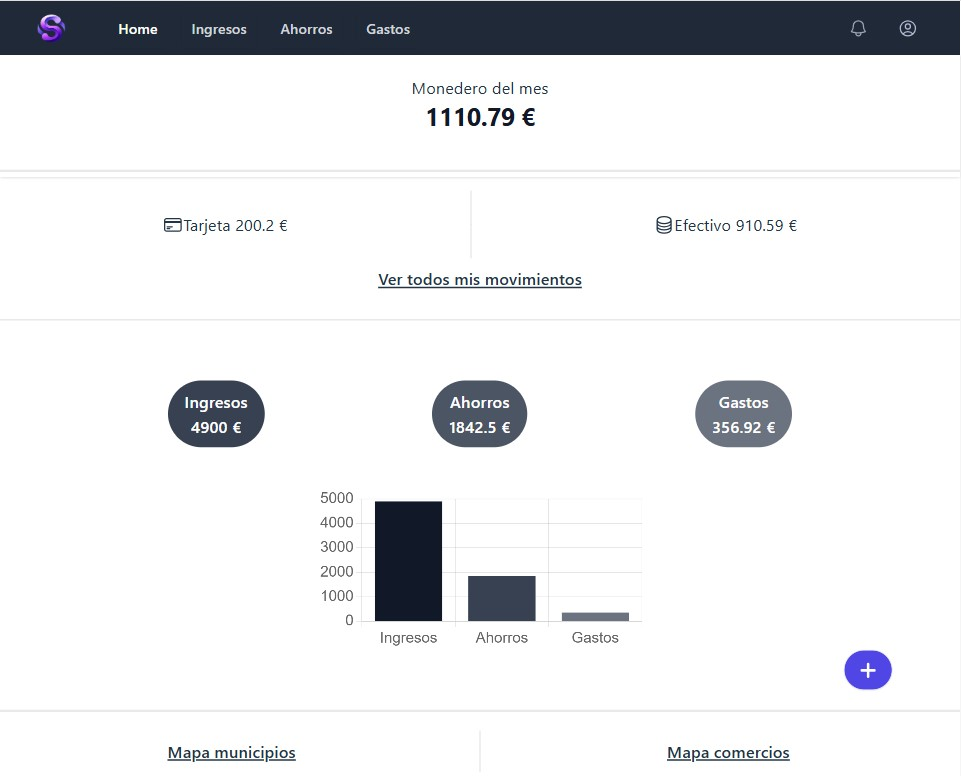
\includegraphics[width=\linewidth]{imagenes/M3-home.jpg}
    \caption{Gráfico de barras en la vista de inicio}
    \label{fig:bar_chart}
\end{figure}

\begin{figure}[ht!]
    \centering
    \begin{minipage}{0.45\textwidth}
        \centering
        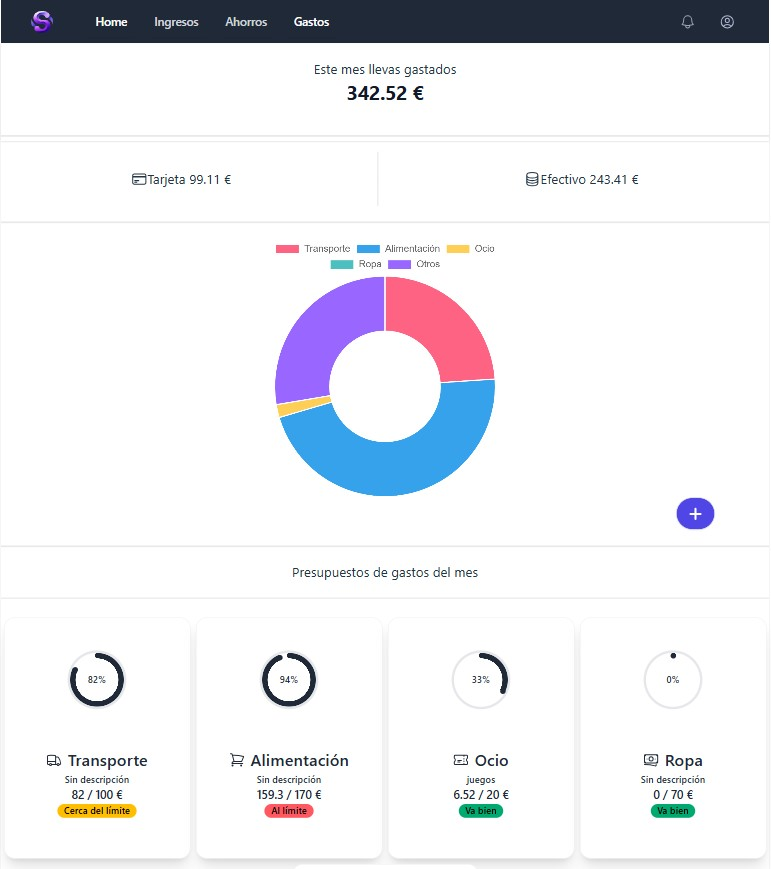
\includegraphics[width=\linewidth]{imagenes/M3-gastos.jpg}
    \end{minipage}\hfill
    \begin{minipage}{0.45\textwidth}
        \centering
        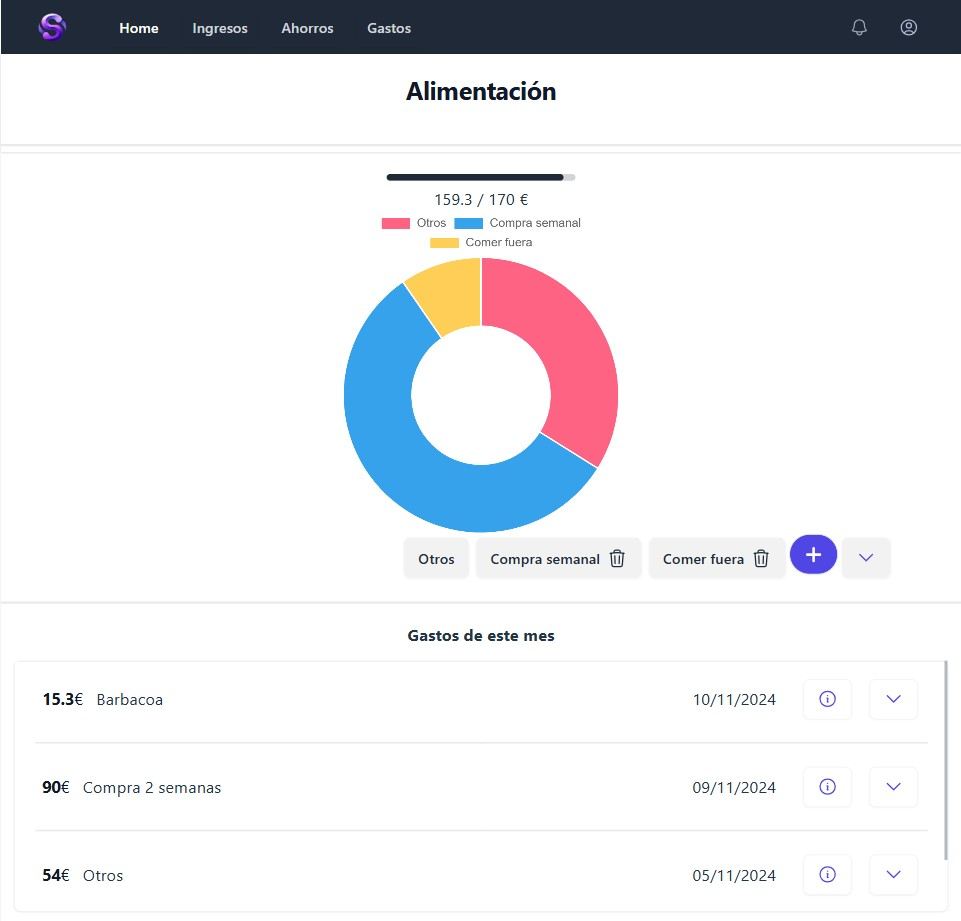
\includegraphics[width=\linewidth]{imagenes/M3-gastos-categoria.jpg}
    \end{minipage}
    \caption{Diagrama de anillo en la vista de gastos y la vista de categoría de gasto}
    \label{fig:doughnut_chart}
\end{figure}

\begin{figure}[ht!]
    \centering
    \begin{minipage}{0.45\textwidth}
        \centering
        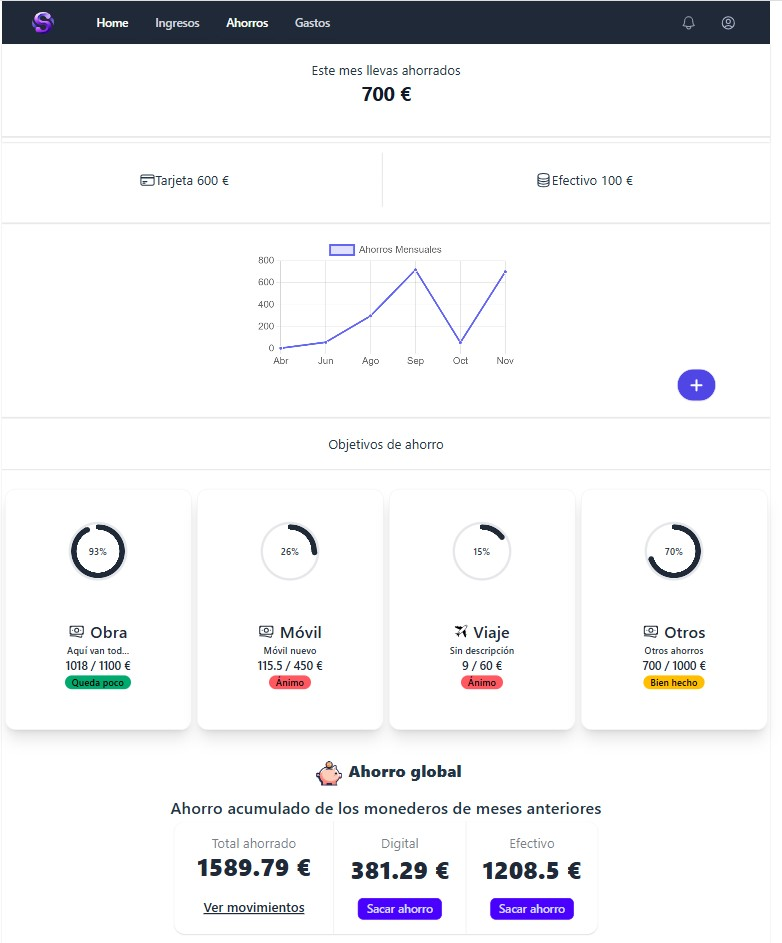
\includegraphics[height=70mm]{imagenes/M3-ahorros.jpg}
    \end{minipage}\hfill
    \begin{minipage}{0.45\textwidth}
        \centering
        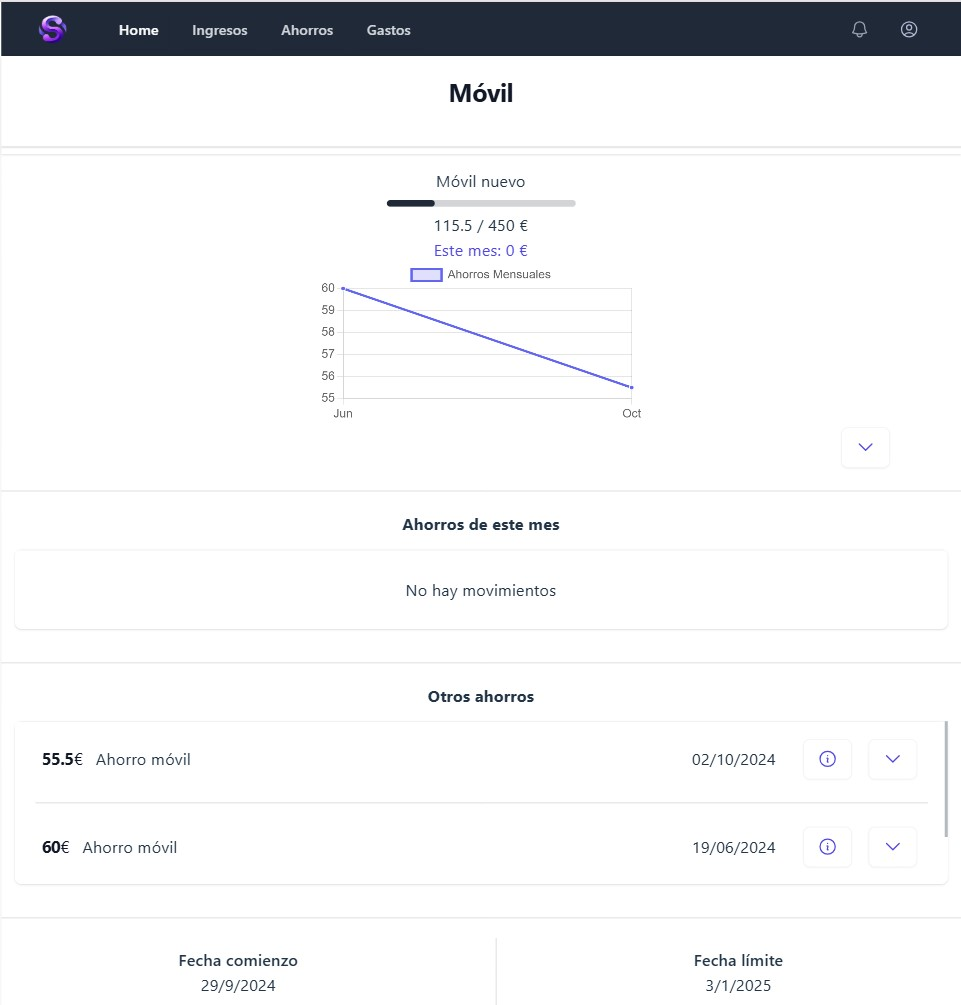
\includegraphics[height=70mm]{imagenes/M3-ahorros-objetivo.jpg}
    \end{minipage}
    \caption{Gráfico de líneas en la vista de ahorros y la vista de objetivo de ahorro}
    \label{fig:line_chart}
\end{figure}


\section{Extracción automática de datos a partir de tickets de compra (basado en OCR): Milestone 4}\label{chap:milestone4}
El reconocimiento del texto de tickets por OCR presenta ciertas limitaciones cuando se emplean fuentes con estilos decorativos, letras cursivas, si la calidad de la imagen no es buena o si el ticket tiene partes que se han comenzado a borrar. Si bien se ha probado con el uso de APIs con versiones gratuitas para comparar la extracción (como \textit{Flashtext} o \textit{OCR.space}), el resultado de la lectura es muy similar al de Tesseract OCR, y se asume en este punto que la extracción de texto no será perfecta.

Dado el propósito de utilizar OCR en la aplicación, no será problema que la precisión no sea del 100\%, ya que el usuario podrá validar los datos si es necesario. Aun así, puesto que el objetivo para el que se usa OCR es procesar el texto obtenido para agilizar la introducción de datos en la aplicación, en el código desarrollado para tal uso, se ha incluido la implementación de numerosas funciones que validan los datos obtenidos. De esta forma (a excepción del campo con el nombre del comercio) \textbf{si no se puede asegurar el relleno correcto de un campo, no se autorellenará en el formulario para evitar un sobreesfuerzo al usuario}.


Al inicio se valora usar alguna herramienta que permita extraer la información relevante de un ticket, sin embargo no se ha encontrado ninguna herramienta gratuita y de acceso ilimitado que lo solucione. 

Se ha planteado la creación de un endpoint en el backend que reciba una imagen de un ticket de compra y devuelva el texto extraído de la imagen, ya procesado y listo para rellenar el formulario de creación de un nuevo gasto. Para ello, se ha creado un componente en React que permite al usuario subir una imagen y enviarla al backend para su procesamiento. Dada una entrada de imagen, la aplicación es capaz de devolver la información útil para rellenar los campos del formulario.

\begin{itemize}
    \item \textbf{Solicitud POST.} El cliente envía el archivo en una solicitud HTTP de tipo POST al endpoint.
    \item \textbf{Guardado del archivo.} El archivo se guarda temporalmente en el servidor.
    \item \textbf{Procesamiento del archivo.} Se comienza el procesamiento a partir de la ruta del archivo guardado.
    \item \textbf{Procesamiento OCR.} Uso de pytesseract para extraer texto del archivo.
    \item \textbf{Extracción de información.} Se procesa el texto extraído para obtener información específica del ticket como el nombre de la tienda, código postal, fecha, método de pago y monto total.
    \item \textbf{Respuesta.} La información extraída se devuelve como respuesta JSON al cliente.
\end{itemize}

Para el procesamiento de las imágenes se ha usado el módulo \textbf{Image} de la librería \textbf{Pillow}, una bifuración de PIL (\textit{Python Imaging Library})\cite{rodrigues202440}. Gracias a la simplicidad de pytesseract y PIL, el proceso de extracción de texto a partir de una imagen es sencillo, por lo que se ha decidido expandir la funcionalidad del script para que pueda procesar tanto imágenes como \textbf{PDFs} (puesto que actualmente algunos comercios envían el ticket de compra al usuario en este formato). Este cambio no supone inconvenientes en el desarrollo, ya que la metodología de extracción de texto es la misma, solo es necesario añadir otra forma de cargar el archivo.

EL código para la extracción de los datos del ticket se ha realizado mediante un script en Python (de acuerdo al lenguaje de programación del backend). La implementación de la lectura de datos de un ticket a partir de una imagen o PDF sigue varios pasos, la funcionalidad del script se puede dividir en las tareas que se describen a continuación.


\subsubsection{Extracción del texto de la imagen}
El módulo \textbf{Image} de la biblioteca \textbf{PIL} permite cargar y manipular imágenes. Se realiza la carga de la imagen desde el archivo almacenado en el servidor y se extrae el texto completo del ticket con la función \textit{image\_to\_string} de \textbf{pytesseract} (Código \ref{cod:leer-imagen}).
    
\begin{lstlisting}[language=Python, caption=Extracción de texto de una imagen, label=cod:leer-imagen]
    from PIL import Image
    import pytesseract

    def get_data_from_image_ticket(file_name):
        image = Image.open(f'app/tests/tickets_images/{file_name}')
        text = pytesseract.image_to_string(image)

        return get_data(text)
\end{lstlisting}

\subsubsection{Extracción del texto del PDF}
Inicialmente la extracción se hace con la biblioteca \textbf{PyMuPDF} por su fama de ser muy rápida en la lectura de PDFs. Con un par de ejemplos se han encontrado problemas en la lectura de los archivos que contenían datos estructurados en columnas, algo usual en los tickets, ya que presentan tablas con los productos comprados. Por ello finalmente se opta por \textbf{PDF Plumber}, una biblioteca de Python que permite extraer directamente texto e información de los PDFs. De la misma forma que con las imágenes, se carga el archivo y se extrae el texto completo del ticket. Se usará esta función en lugar de la anterior cuando la extensión del archivo sea PDF (Código \ref{cod:leer-texto}).

\begin{lstlisting} [language=Python, caption=Extracción de texto de un PDF, label=cod:leer-texto]
    import pdfplumber

    def get_data_from_pdf_ticket(file_name):
        text = ""
        with pdfplumber.open(f'app/tests/tickets_PDFs/{file_name}') as pdf:
            for page in pdf.pages:
                page_text = page.extract_text()
                if page_text:
                    text += page_text + '\n'
        
        return get_data(text)
\end{lstlisting}

\subsubsection{Análisis de los elementos en un ticket}
Una vez obtenida la cadena de texto, ya sea desde la imagen o el PDF, se inicia el proceso de identificación de los componentes en un ticket. Este proceso comienza con un análisis exhaustivo de diversos tickets por parte del desarrollador para determinar la información relevante que se puede extraer porque se presenta de forma general en ellos: nombre del comercio, dirección, código postal, nombre del municipio, NIF, fecha, método de pago e importe total (Figura \ref{fig:componentes_ticket}).

De ellos, se valora cuáles serían de utilidad para completar el formulario de creación de una transacción de gasto (se puede ver la vista del formulario en la Figura \ref{fig:formulario_gasto}) e implementar el mecanismo para extraerlos.

\begin{figure}[ht!]
    \centering
    \begin{minipage}{0.45\textwidth}
        \centering
        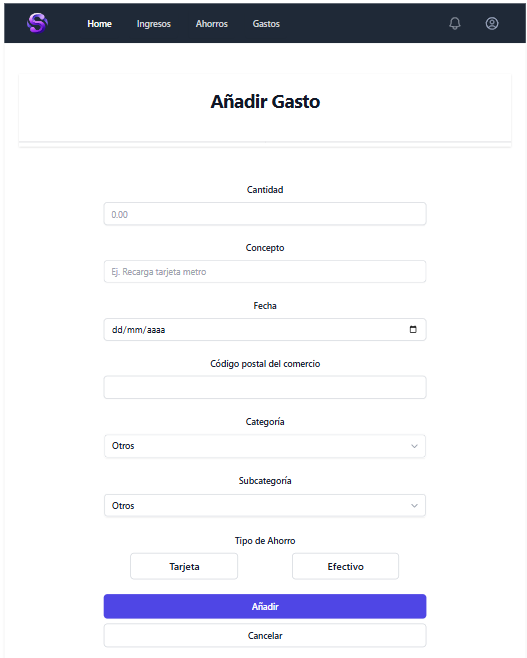
\includegraphics[height = 70mm]{imagenes/formulario_gasto.png}
        \caption{Formulario de creación de un gasto}
        \label{fig:formulario_gasto}
    \end{minipage}\hfill
    \begin{minipage}{0.45\textwidth}
        \centering
        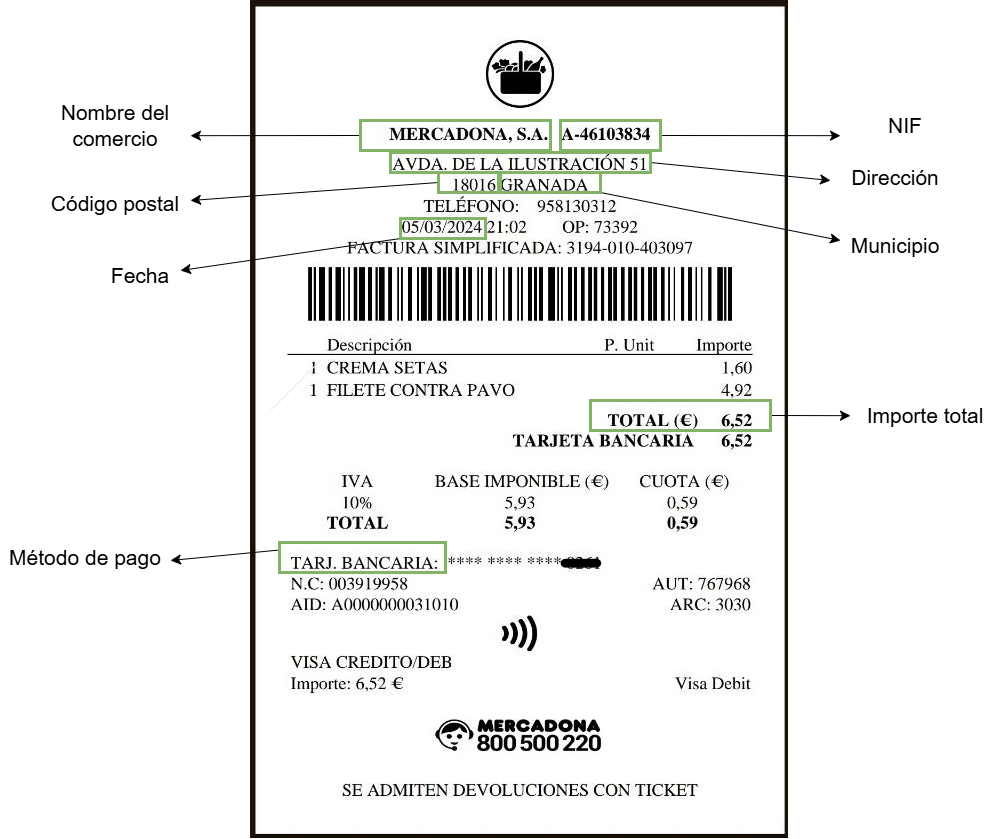
\includegraphics[height = 70mm]{imagenes/componentes_ticket.png}
        \caption{Componentes de un ticket}
        \label{fig:componentes_ticket}
    \end{minipage}
\end{figure}

\subsubsection{Extracción de campos}
Dado que los tickets suelen ser textos breves, en la mayoría de casos se usan de expresiones regulares (regex) para buscar y extraer información específica. Las expresiones regulares son especialmente útiles para esta tarea, ya que permiten definir patrones precisos de búsqueda y son rápidas en volúmenes reducidos de texto. Así, se crean funciones específicas para identificar y extraer cada dato relacionado con un campo del formulario.

Cada función es llamada desde una función principal (Código \ref{cod:dictionary}) que recibe el texto extraído del ticket y devuelve un diccionario con los campos identificados y el valor extraído. En caso de no encontrar un campo, se devuelve en él valor 'desconocido'.

\begin{lstlisting} [language=Python, caption=Extracción los campos del ticket, label=cod:dictionary]
    # returns a dictionary with ticket data
    def get_data(text):
        text = text.lower()

        payment_method = get_payment_method(text)
        date = get_date(text)
        shop_data = get_shop_data(text)
        total_amount = get_total_amount(text)

        ticket_data = {
            'shop_name': shop_data['shop_name'],
            'shop_postal_code': shop_data['postal_code'],
            'date': date,
            'payment_method': payment_method,
            'total_amount': total_amount,
        }

        return ticket_data
\end{lstlisting}


\begin{itemize}
    \item \textbf{Método de pago.} Se determina si el método de pago es en efectivo o tarjeta, o si es desconocido. Primero busca palabras clave directas que identifiquen un método u otro como que aparezca la cadena 'efectivo'. Si no las encuentra cuenta las ocurrencias de palabras clave relacionadas para hacer una determinación basada en la frecuencia de estas palabras (Código \ref{cod:pago}).
    
    \begin{lstlisting}[language=Python, caption=Extracción del método de pago en un ticket, label=cod:pago]
    # returns 'tarjeta', 'efectivo' or 'desconocido' if not found
    def get_payment_method(text):
        payment_method = 'desconocido'
    
        if 'tarjeta' in text:
            payment_method = 'tarjeta'
        elif 'efectivo' in text or 'contado' in text:
            payment_method = 'efectivo'
        else:
            count_tarjeta = 0
            count_efectivo = 0
    
            keywords_tarjeta = ['visa', 'mastercard', 'debito', 'debit', 'credito', 'credit', 'contactless', 'nfc', 'cuenta','caixabank', 'bbva', 'trj', 'jeta', 'tarj', 'tanjeta']
            keywords_efectivo = ['cambio', 'entrega', 'entregado', 'efect', 'entr', 'cont']
    
            count_tarjeta = sum(text.count(keyword) for keyword in keywords_tarjeta)
            count_efectivo = sum(text.count(keyword) for keyword in keywords_efectivo)
    
            if count_tarjeta >= 2 and count_tarjeta > count_efectivo:
                payment_method = 'tarjeta'
            elif count_efectivo >= 2 and count_efectivo > count_tarjeta:
                payment_method = 'efectivo'
                
        return payment_method
    \end{lstlisting}

    \item \textbf{Fecha.} Se busca la fecha, que puede aparecer en diferentes formatos, se han contemplado varios formatos posibles (\textit{dd\_mm\_yyyy, dd\_mm\_yy, yyyy\_mm\_dd}). Primero elimina los espacios en blanco del texto y luego intenta extraer la fecha en cada uno de los formatos mencionados, estableciendo prioridad en los intentos, ya que el formato de fecha más frecuente en España es \textit{dd\_mm\_yyyy}. Si no se encuentra una fecha en ninguno de los formatos, devuelve 'desconocido'. Para cada formato se comprueba la validez de la fecha, y que no se extraiga más de una fecha en el texto (ya que en algunos tickets se muestra la fecha límite para devoluciones), si no se cumple alguna de estas condiciones se devuelve 'desconocido' (Código \ref{cod:fecha}).

    \begin{lstlisting} [language=Python, caption=Extracción la fecha en un ticket, label=cod:fecha]
    # returns date with dd/mm/aaaa format o 'desconocido' if not found
    def get_date(text):
        date = 'desconocido'
        text = text.replace(' ', '')

        date = get_date_dd_mm_yyyy(text)
        if date == 'desconocido':
            date = get_date_dd_mm_yy(text)   
            if date == 'desconocido':
                date = get_date_yyyy_mm_dd(text)

        return date
    \end{lstlisting}

    \item \textbf{Datos del comercio.} Se extrae información relevante sobre una tienda, específicamente el nombre de la tienda y el código postal. Utiliza funciones auxiliares (\textit{get\_postal\_code, get\_street, get\_shop\_name}) para obtener estos datos y los organiza en un diccionario que luego devuelve (Código \ref{cod:shop}).
    
    Para las extracciones de los campos concretos se han usado expresiones regulares.  

    \begin{lstlisting} [language=Python, caption=Extracción de los datos del comercio, label=cod:shop]
    # returns a dictionary with shop data
    def get_shop_data(text):
        postal_code = get_postal_code(text)
        street = get_street(text, postal_code)
        shop_name = get_shop_name(text)

        shop_data = {
            'shop_name': shop_name,
            'postal_code': postal_code,
        }
        return shop_data
    \end{lstlisting}

\subitem \textbf{Código postal}. Se busca un patrón de cinco dígitos aislado en el texto, se asume que en la mayoría casos este será el código postal de la tienda. Si no se encuentra, devuelve 'desconocido' (Código \ref{cod:cp}). \label{item:codigo_postal}
    \begin{lstlisting} [language=Python, caption=Extracción del código postal, label=cod:cp]
    # returns postal code or 'desconocido' if not found
    def get_postal_code(text):
        postal_code = 'desconocido'

        match = re.search(r'\n[\s\n]*\d{5}[\s\n.-]', text)
        if match:
            match_postal_code = re.search(r'\d{5}', match.group(0))
            postal_code = match_postal_code.group(0)

        return postal_code
    \end{lstlisting}


\subitem La función para el \textbf{nombre de la tienda} toma un texto y una calle como entrada y trata de extraerlo: busca patrones específicos que coincidan con nombres de tiendas que terminan en \textit{S.A.} o \textit{S.L.} y si esa búsqueda no encuentra coincidencias, toma las primeras dos líneas del texto. Si encuentra una coincidencia elimina la calle (dirección) si se ha añadido erróneamente dentro del nombre. Finalmente, devuelve el nombre de la tienda o 'desconocido' si no se encontró ninguna coincidencia (Código \ref{cod:name}).
    \begin{lstlisting} [language=Python, caption=Extracción del nombre de la tienda, label=cod:name, literate={á}{{\'a}}1 {é}{{\'e}}1 {í}{{\'i}}1 {ó}{{\'o}}1 {ú}{{\'u}}1 {ñ}{{\~n}}1 {Á}{{\'A}}1 {É}{{\'E}}1 {Í}{{\'I}}1 {Ó}{{\'O}}1 {Ú}{{\'U}}1 {Ñ}{{\~N}}1]
    # returns shop name or 'desconocido' if not found
    def get_shop_name(text, street):
        shop_name = 'desconocido'

        text = re.sub(r'\r;)(', ' ', text)

        match = re.search(r'[a-zá-ú]+.*[sS]\.[aAlL]+', text) # S.A. (Sociedad Anónima) // S.L. (Sociedad Limitada)

        if not match:
            match = re.search(r'[a-zá-ú].+\n.*\n', text) # first two lines
        if match:
            shop_name = match.group(0).replace('\n', ' ').replace('\r', ' ')
            if street in shop_name:
                shop_name = shop_name.replace(f'{street}', '')

        return shop_name
    \end{lstlisting}

En esta extracción se presenta la dificultad de que los nombres de tiendas no suelen seguir un patrón claro, en el texto del ticket es fácil perder la referencia de qué es el nombre de la tienda, qué es la dirección o la descripción de un artículo. Por ello se ha decidido extraer el nombre por su posición al inicio del texto si no se encuentra un patrón que lo identifique. Además, como alternativa al uso de patrones se han probado bibliotecas de procesamiento de lenguaje natural como \textit{spaCy} para extraer entidades (como nombres de tiendas o ciudades) usando un modelo preentrenado en español. Se intenta también
la extracción con \textit{Flashtext} para buscar coincidencias de nombres de tiendas en una lista de
comercios conocidos, sin conseguir mejores resultados. La extracción del NIF se ha resuelto con patrones específicos,
y aunque se ha considerado relacionarlo con el nombre del comercio a través de APIs,
su uso se descarta para este proyecto debido a las restricciones en el volumen de
consultas que ofrecen los planes gratuitos.

    \item \textbf{Importe total.} Este procesamiento es el más complejo, ya que se buscan cadenas coincidentes con el formato esperado, y en este caso, todos los números del ticket tienen el mismo formato. Esto puede generar ambigüedad en la extracción del importe total.

    El aspecto clave para conseguir la cantidad total reside precisamente en esta palabra de la que va acompañada: 'total'. Se busca la palabra 'total' en el texto seguida de un número con decimales y posiblemente una representación de la divisa: el símbolo \textit{€}, la palabra \textit{euro} o simplemente la letra \textit{e}.  Si no se encuentra se realizan búsquedas alternativas, con la palabra 'importe', 'venta' o partes de ellas. Las coincidencias obtenidas se almacenan en una lista de Python que se irá depurando, eliminando de ella los precios que indican un total de IVA, un total de descuento, o si se encuentra un número al final de línea (cuando no hay descuentos) mayor que los de la lista de candidatos (Código \ref{cod:total}). De modo que en casos como el de la Figura \ref{fig:get_total_amount_peculiaridades} se extraería el importe total de 29,96 porque se descartaría 24,00 de la lista de candidatos.

    \begin{figure}[ht!]
        \centering
        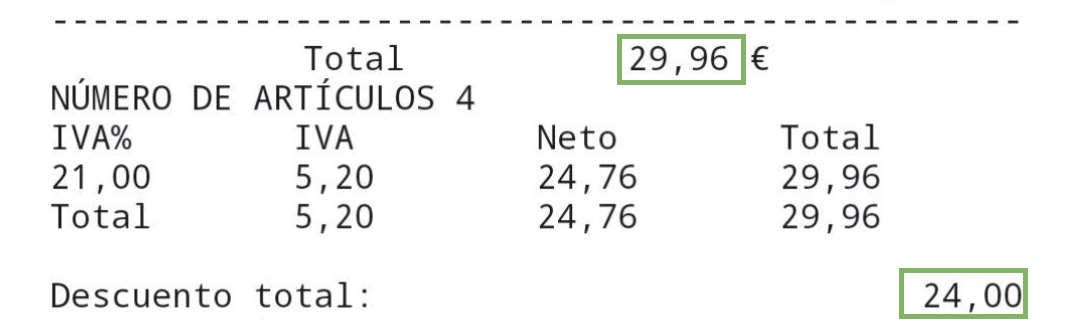
\includegraphics[height=30mm]{imagenes/get_total_amount_peculiaridades.png}
        \caption{Ticket con descuento}
        \label{fig:get_total_amount_peculiaridades}
    \end{figure}

Texto leído del fragmento de la Figura \ref{fig:get_total_amount_peculiaridades}
    \begin{lstlisting}[literate={€}{{\euro}}1 {á}{{\'a}}1 {é}{{\'e}}1 {í}{{\'i}}1 {ó}{{\'o}}1 {ú}{{\'u}}1 {ñ}{{\~n}}1]
        \n\n \n\n \n\n \n\ntotal 29,96 €\nnumero de articulos 4\niva% iva neto total\n21,00 5,20 24,76 29,96\ntotal 5,20 24,76 29,96\ndescuento total: 24,00
    \end{lstlisting}

    \begin{lstlisting} [language=Python, caption=Extracción del importe total, label=cod:total]
    # returns total amount or 'desconocido' if not found
    def get_total_amount(text):
        total_found = False
        total_amount ='desconocido'
        total_from_eol_prices = 0
        total_from_candidates = 0
        percentage_prices = get_iva_prices(text)
        discount_prices = get_discount_prices(text)

        invalid_prices = percentage_prices + discount_prices

        if not discount_prices:
            eol_prices = get_eol_prices(text, invalid_prices)         
            if eol_prices:
                total_from_eol_prices = max(eol_prices)
        
        total_prices = get_total_prices(text, invalid_prices)

        if total_prices:
            total_found = True
            total_from_candidates = max(total_prices)      
        
        if total_found:
            if total_from_candidates >= total_from_eol_prices:
                total_amount = str(total_from_candidates)

        return total_amount
    \end{lstlisting}
\end{itemize}


\subsubsection{Problemas encontrados}
La identificación de cadenas de texto sin patrones claros como el nombre de la tienda comprometen la precisión de los resultados. La dificultad se agrava debido a que los tickets contienen caracteres especiales, saltos de línea y símbolos que, al mezclarse en el texto, dificultan identificar palabras o frases completas, así como ciertas tipografías que usan los nombres de comercios. 

El resto de los campos del formulario están sometidos a validaciones estrictas para asegurar la calidad de los datos; si no cumplen con los requisitos, el sistema no registra los valores. Este enfoque prioriza la precisión, de modo que el usuario evite corregir manualmente campos incorrectos. A diferencia del resto, para simplificar el proceso de entrada de datos, el campo 'concepto' de gasto se rellena con el nombre del comercio aunque no sea una coincidencia perfecta, ya que solo sirve como referencia identificativa de la transacción.

El resto de información que se ha procesado, pero no ha sido relevante o no ha sido posible extraerla con precisión, se ha descartado. Por ejemplo, la dirección del comercio (calle y municipio), el NIF, el IVA o si había descuentos. Los métodos implementados están disponible en el repositorio donde se aloja el proyecto, aunque se ha decidido no incluirlos en la aplicación para no sobrecargar al usuario con información innecesaria, manteniendo así la simplicidad de la interfaz.


\subsubsection{Pruebas}
Se han guardado 24 tickets de diferentes comercios en formato de texto (usando las funciones de extracción de texto implementadas) para realizar pruebas con el script de extracción de datos. Estos tickets sirven como base para realizar pruebas controladas que permiten medir la capacidad del script para identificar correctamente los campos relevantes. Para una representación más realista, se han incluido tickets en formato tanto procedentes de imagen como PDF, procurando que las muestras tengan variedad de fuentes y estilos de texto, así como tickets con errores de impresión o deterioro.

Se emplea \textbf{pytest} para desarrollar pruebas unitarias para cada una de las funciones encargadas de extraer los campos específicos del ticket, como el nombre del comercio, el importe total, la fecha y otros datos de interés. Cada función se prueba con múltiples casos representativos, verificando que los valores devueltos sean los esperados. Esto ha permitido observar cómo respondía el código desarrollado ante diferentes formatos y disposición de elementos en los tickets (Código \ref{cod:test_fechas}). A través de estas pruebas, la implementación se ha ido ajustando progresivamente para maximizar la precisión en la extracción de datos.

\begin{lstlisting} [language=Python, caption=Tests de extracción de fechas, label=cod:test_fechas]
    # returns total amount or 'desconocido' if not found
    def test_get_date_dd_mm_yy():
        expected = ["desconocido", "12/06/2024", "desconocido", "desconocido", "desconocido", "16/08/2024",
                    "15/06/2024", "24/06/2024"]
        tickets_dd_mm_yy = [text[4], text[6], text[7], text[10], text[18], text[19],
                            text[21], text[22]]
        i = 0
        for ticket in tickets_dd_mm_yy:
            with open(f'{base_path}{ticket}', 'r') as file:
                ticket_str = file.read().lower()
                assert get_date(f'{base_path}{ticket_str}') == expected[i]
                i += 1

    def test_get_date_yyyy_mm_dd():
        # on ticket: 3(2024-04-23)
        expected = ["23/04/2024", "desconocido"]
        tickets_yyyy_mm_dd = [text[3]]
        i = 0
        for ticket in tickets_yyyy_mm_dd:
            with open(f'{base_path}{ticket}', 'r') as file:
                ticket_str = file.read().lower()
                assert get_date(f'{base_path}{ticket_str}') == expected[i]
                i += 1

    def test_get_date_mix():
        # on: (09/05/21) -> solo fechas de 2024 en adelante
        expected = ["01/01/2024", "02/02/2024", "03/03/2024", 
                    "04/04/2024", "05/05/2024", "06/06/2024", 
                    "07/07/2024", "08/08/2024", "09/09/2024","desconocido"]
        dates_mix = ["srd01/01/2024", "rtnjs 02-02-2024", "rtrju 03.03.2024", 
                    "03948n 04/04/24", "asff05-05-24", "06.06.24dvgsd", 
                    "2024-07-07", "2024/08/08 sdr", "2024.09.09 999", "09/05/21"]
        i = 0
        for date in dates_mix:
            assert get_date(date) == expected[i]
            i += 1
\end{lstlisting}

\subsubsection{Conclusiones}
El uso de OCR para la extracción de datos de tickets ha sido un reto interesante y ha permitido mejorar la experiencia del usuario en la aplicación. Aunque la precisión de la extracción no es del 100\%, el script desarrollado ha demostrado ser capaz de extraer información relevante de los tickets de compra, lo que facilita la introducción de gastos en la aplicación. En cuanto a la implementación, se ha logrado un buen equilibrio entre la precisión y la velocidad de procesamiento, lo que permite al usuario ahorrar tiempo y esfuerzo en la introducción manual de gastos y aumenta la probabilidad de que los usuarios completen todos los campos de las transacciones.

En la Tabla \ref{tab:pruebas_extraccion_datos} se muestra un resumen de algunos resultados obtenidos en las pruebas realizadas con el script de extracción de datos de tickets. Se puede observar que la precisión de la extracción varía según el campo y el formato del ticket, pero en general, el script ha demostrado ser capaz de identificar correctamente los campos relevantes en la mayoría de los casos.

\begin{landscape}
    \begin{table}[]
    \begin{tabular}{|p{3cm}|p{3cm}|l|l|l|l|p{3cm}|l|}
    \hline
    \textbf{\begin{tabular}[c]{@{}l@{}}Nombre \\Comercio\end{tabular}} & \textbf{\begin{tabular}[c]{@{}l@{}}Nombre Leído\\ (concepto)\end{tabular}} & \textbf{Código Postal} & \textbf{Total} & \textbf{Fecha} & \textbf{\begin{tabular}[c]{@{}l@{}}Método\\ de Pago\end{tabular}} & \textbf{\begin{tabular}[c]{@{}l@{}}Observaciones \\sobre el Ticket\end{tabular}} & \textbf{\begin{tabular}[c]{@{}l@{}}Errores \\Extracción \\de Campos\end{tabular}} \\ \hline
    Ikea Ibérica, s.a. & Tkea ibfrica, s.a & 18100 & 2.99 & 05/08/2024 & Tarjeta & \begin{tabular}[c]{@{}l@{}}Formato fecha:\\ 05.08.24\end{tabular} & \\ \hline
    \begin{tabular}[c]{@{}l@{}}Ikea Ibérica, s.a. \\Capt. Pantalla\end{tabular} & Ikea iberica, s.a. & 18100 & 103.0 & 26/03/2024 & Tarjeta &  &  \\ \hline
    Casa del Libro & Liente & desconocido & 9.85 & 23/04/2024 & Tarjeta & \begin{tabular}[c]{@{}l@{}}Formato fecha:\\ 2024-04-23\end{tabular} & \begin{tabular}[c]{@{}l@{}}Lectura nombre\\ No lee C.P.\end{tabular}\\ \hline
    Lefties & Lefties & desconocido & 17.99 & 01/02/2024 & Tarjeta & No incluye C.P. &  \\ \hline
    Primor & Megapr i mor, s.l & 18100 & 4.3 & 12/06/2024 & Tarjeta & \begin{tabular}[c]{@{}l@{}}Formato fecha:\\ 12/06/24\end{tabular} &  \\ \hline
    Mercadona, s.a. & Mercadona, s.a & 18016 & \begin{tabular}[c]{@{}l@{}}desco-\\nocido\end{tabular} & 17/06/2024 & Tarjeta &  &  \\ \hline
    \begin{tabular}[c]{@{}l@{}}Mercadona, s.a. \\Capt. Pantalla\end{tabular} & Mercadona, s.a & 18016 & 6.52 & 05/03/2024 & Tarjeta &  & No lee C.P.. \\ \hline
    Cervecería Ecu & Cerveceria ecu §2.521.648k & 18008 & 22.3 & 23/06/2024 & Efectivo &  & Lectura nombre. \\ \hline
    \begin{tabular}[c]{@{}l@{}}HyM \\Capt. Pantalla\end{tabular} & Comprarent... q sl © & 18100 & 2.99 & 24/06/2024 & Tarjeta & \begin{tabular}[c]{@{}l@{}}Precio descuento\\mayor a total\end{tabular} & Lectura nombre \\ \hline
    Margaritas Blancas & Margaritas blancas & desconocido & 6.5 & 27/04/2024 & Efectivo & No incluye  C.P. &  \\ \hline
    \begin{tabular}[c]{@{}l@{}}Carrefour\\PDF\end{tabular} & \begin{tabular}[c]{@{}l@{}}Centros comerciales\\ carrefour s.a\end{tabular} & desconocido & 49.78 & 19/08/2024 & Tarjeta & \begin{tabular}[c]{@{}l@{}}PDF. No tiene C.P.\\(compra online)\end{tabular} &  \\ \hline
    \begin{tabular}[c]{@{}l@{}}Mercadona, s.a\\PDF\end{tabular} & Mercadona, s.a & 18016 & 3.5 & 09/04/2024 & Tarjeta & \begin{tabular}[c]{@{}l@{}}PDF recibo de\\ compra física\end{tabular} &  \\ \hline
    \end{tabular}
    \caption{Pruebas de extracción de datos en tickets de diferentes comercios.}
    \label{tab:pruebas_extraccion_datos}
    \end{table}
\end{landscape}
    


\section{Localización de comercios (basado en GPS) y generación de resúmenes de gastos localizados en mapas: Milestone 5} \label{chap:milestone5}
En este milestone se han desarrollado las funcionalidades de la aplicación que permiten la incorporación de tiendas, así como la creación de una nueva visualización en mapas del análisis mensual de gastos que realizan los usuarios (agrupándolos por localidades o tiendas).

Continuando con la simplicidad en la introducción de gastos, se ha decidido no hacer obligatorios los campos de código postal y tienda en el formulario de gastos, por lo que el usuario podrá elegir:

\begin{itemize}
    \item Si desea introducir el código postal o no. Este campo se auto rellenará si se ha podido obtener del ticket, por lo que en la mayoría de los casos el usuario no tendrá que introducirlo manualmente. Si se ha completado, el usuario tendrá disponible la representación en el mapa del total de gastos mensuales en esa localidad. 
    
    \item Si desea introducir la tienda o no. Tendrá que haberse rellenado el código postal para poder seleccionar una tienda de la lista ofrecida por la aplicación. Si se ha completado, el usuario tendrá disponible la representación en el mapa del total de gastos mensuales en esa tienda.
\end{itemize}

A lo largo de esta sección se describen los endpoints desarrollados para obtener los datos necesarios que permitan la representación de los gastos en el mapa de España. Los resultados de las consultas a estos endpoints se devuelven en formato JSON y se representa en un componente frontend que, usando la biblioteca \textit{react-leaflet}, muestra un mapa con los puntos de gasto representados en él. Adicionalmente, se han realizado llamadas a la API de Overpass para obtener información sobre los comercios cercanos a una ubicación concreta.


\subsection{Mapa de gastos por localidad}
El código postal es un dato que aparece frecuentemente en los tickets de compra. Sigue un patrón sencillo por lo que es probable que se pueda extraer con precisión de forma automática con el mecanismo implementado en el Milestone 4 \ref{item:codigo_postal}. 


\subsubsection{Solución al problema de códigos postales}
Para evitar inconsistencias (o un procesamiento excesivamente dependiente de APIs externas), se ha creado una nueva tabla (independiente del resto) en la base de datos PostgreSQL con toda la información necesaria de localidades y códigos postales de España. Esta tabla crea tomando como base un fichero CSV descargado de la web \textit{CentraldeComunicación.es} que contiene una lista de códigos postales de España y sus correspondientes coordenadas geográficas. A esta información se le añaden los datos de provincia (nombre y código) extraídos de la \textit{Relación de municipios y sus códigos por provincias} del 1 de enero de 2024 publicada por el Instituto Nacional de Estadística. Por último, para solventar el problema de los códigos postales diferentes para una misma localidad, se ha creado una columna en la tabla que asigna como elegido solo un código postal por localidad; entendiendo una localidad como una región de nombre único que se determinará por la columna \textit{entidad\_singular\_nombre} de la tabla de municipios que usa la aplicación (como se muestra en la Figura \ref{fig:CSV_municipios}). De esta forma, aunque cada transacción guarde un código postal diferente, se agruparán (y representarán) en una única zona en el mapa si se considera que pertenecen a la misma localidad.

Ejemplo: si un usuario realiza una compra en un supermercado en la localidad de Granada, y el ticket recoge el código postal 18008, y otro usuario realiza una compra en un supermercado en la misma localidad, pero el ticket recoge el código postal 18006, ambas transacciones se agruparán en el mapa en la localidad de Granada, representando el total de gastos en esa localidad. Para determinar las coordenadas geográficas asociadas a la localidad de Granada se tomarán la latitud y longitud del código postal 18001 porque en la tabla ese código es el elegido para extraer las coordenadas (columna \textit{coords\_elegidas}) de la localidad de Granada.

\begin{figure}[ht!]
    \centering
    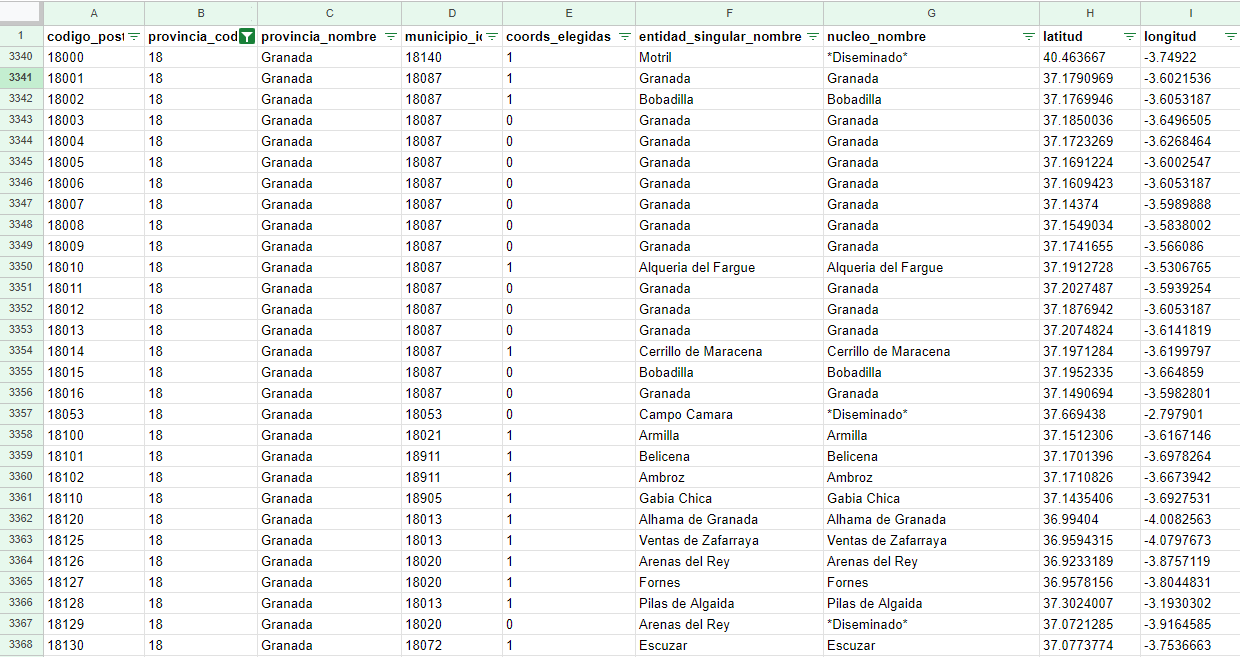
\includegraphics[height=70mm]{imagenes/municipios_cp.png}
    \caption{CSV con la información de códigos postales para la base de datos}
    \label{fig:CSV_municipios}
\end{figure}


\subsubsection{Visualización de los gastos en el mapa}
Para la representación de los gastos en el mapa se necesitan analizar las transacciones correspondientes a operaciones de gasto realizadas en el mes actual y extraer las coordenadas geográficas de las localidades para representarlos en un punto concreto en el mapa. 

Como solución se ha implementado un endpoint (Figura \ref{fig:api-expenses_by_location}) en el backend que obtiene los gastos por ubicación para el mes actual. Primero filtra las transacciones del mes y año actuales, agrupadas por código postal. Del resultado extrae cada código postal con el total de gastos asociado a él y le añade las coordenadas y nombres de localidades. Finalmente, devuelve una lista de gastos con coordenadas y nombres de entidades (Código \ref{cod:map-local}).

\begin{lstlisting} [language=Python, caption=Endpoint para obtener los gastos por localidad, label=cod:map-local]
@app.get("/expenses_by_location", tags=["Map"], status_code=status.HTTP_200_OK)
def get_expenses_by_location(db: Session = Depends(get_db)):
    current_month = datetime.now().month
    current_year = datetime.now().year

    expenses_by_location_query = db.query(
        Transaction.shop_location_pc,
        func.coalesce(func.sum(Transaction.amount), 0).label('current_amount_spent')
    ).filter(
        Transaction.shop_location_pc != None,
        extract('month', Transaction.insert_date) == current_month,
        extract('year', Transaction.insert_date) == current_year
    ).group_by(Transaction.shop_location_pc).all()

    expenses_by_location = [row._asdict() for row in expenses_by_location_query]

    expenses_with_coordinates = []
    for expense in expenses_by_location:
        postal_code = expense['shop_location_pc']
        coordinates = get_location_by_postal_code(postal_code, db)
        if coordinates != {"desconocido"}:
            existing_expense = next((exp for exp in expenses_with_coordinates if exp['entidad_nombre'] == coordinates['entidad_nombre']), None)
            if existing_expense:
                existing_expense['current_amount_spent'] += expense['current_amount_spent']
                existing_expense['postal_codes'].append(postal_code)
            else:
                expense_by_loc = {
                    'postal_codes': [postal_code],
                    'latitude': coordinates['latitude'],
                    'longitude': coordinates['longitude'],
                    'entidad_nombre': coordinates['entidad_nombre'],
                    'current_amount_spent': expense['current_amount_spent']
                }
                expenses_with_coordinates.append(expense_by_loc)

    return expenses_with_coordinates
\end{lstlisting}

\begin{figure}[ht!]
    \centering
    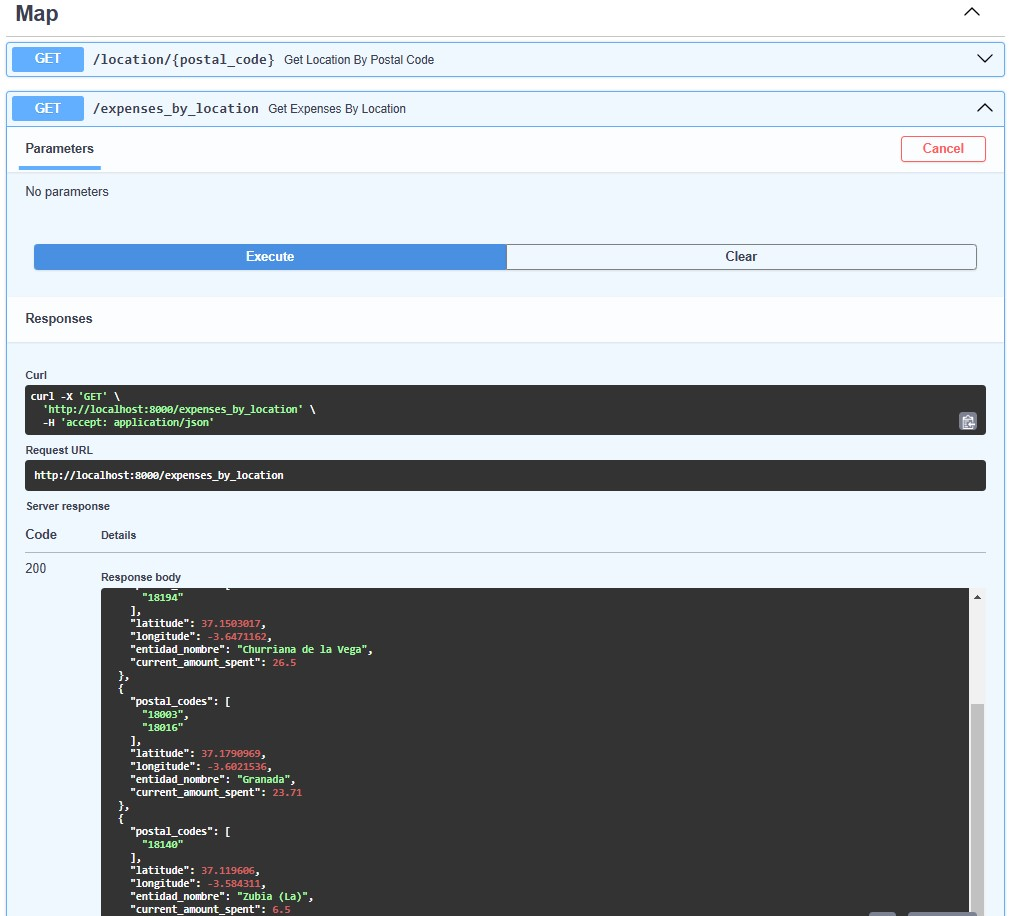
\includegraphics[width=\linewidth]{imagenes/api-expenses_by_location.jpg}
    \caption{Prueba del endpoint \textit{expenses\_by\_location} en la API de FastAPI a través de Swagger}
    \label{fig:api-expenses_by_location}
\end{figure}

\subsection{Mapa de gastos por comercio}
Para ofrecer un análisis geográfico más detallado de los gastos, se ha implementado la visualización sobre el mapa de gastos por tienda. Para ello, en los formularios de introducción de gastos se hizo visible un campo (no usado hasta el momento) para que el usuario pueda introducir la tienda donde realizó la compra. 

Este campo se completa seleccionando un item sobre una lista de tiendas predefinidas, evitando así la introducción manual de la dirección de la tienda y por tanto el sobresfuerzo del usuario. Además, para facilitar la selección de la tienda, se ha implementado un componente en el frontend de un pequeño mapa para que el usuario verifique la ubicación de la tienda seleccionada.

Las información de tiendas se recoge en la base de datos en una tabla que se irá construyendo a medida que los usuarios vayan introduciendo comercios en la aplicación.


\subsubsection{Introducción de un comercio en la aplicación}
El usuario puede introducir una tienda en la aplicación de dos formas: por geolocalización o por búsqueda.

Ambos métodos parten del código postal introducido por el usuario en el formulario de gastos. El proceso para encontrar las tiendas difiere en la forma de obtener las coordenadas con las que iniciar la búsqueda. Cuando se consiguen dichas coordenadas, se construye una consulta en el formato de de Overpass QL para buscar puntos de interés (nodos) que coincidan con el criterio de búsqueda que se haya configurado. La consulta se envía a la API de Overpass y se obtiene una respuesta en formato JSON con los resultados de la búsqueda. Devuelve información de establecimientos de la que se obtienen las coordenadas, calle, nombre e identificador del elemento para introducirlo, junto con el código postal, en la base de datos, creando una nueva entrada en la tabla de tiendas por medio de un endpoint de la API de \textit{SIGMA}.

\begin{itemize}
    \item \textbf{Identificación de un comercio con buscador}\\    
    En este caso, la consulta en el Código \ref{cod:comercio-busc} define diferentes filtros de búsqueda para encontrar elementos en OpenStreetMap con atributos que coincidan con el término de búsqueda (\textit{searchStr}) y estén ubicados en el radio especificado (\textit{meters} alrededor de \textit{lat, lon}). Teniendo en cuenta que las coordenadas parten de un código postal, el radio debe ser lo suficientemente generoso para abarcar la zona completa (aunque suponga exceder el área real del código postal). Siendo:
    \subitem \textit{searchStr} el término de búsqueda introducido por el usuario
    \subitem \textit{meters} la distancia en metros alrededor de la ubicación del usuario
    \subitem \textit{lat, lon} las coordenadas geográficas asociadas al \textbf{código postal} completado en el formulario.
    
    \begin{lstlisting} [language=Python, caption=Consulta de Overpass QL con término de búsqueda, label=cod:comercio-busc]
    const overpassQuery = `
        [out:json];
        (
        node["name"~"${capitalize(searchStr)}"](around:${meters}, ${lat}, ${lon});
        node["shop"~"${capitalize(searchStr)}"](around:${meters}, ${lat}, ${lon});
        node["amenity"~"${capitalize(searchStr)}"](around:${meters}, ${lat}, ${lon});
        node["addr:street"~"${capitalize(searchStr)}"](around:${meters}, ${lat}, ${lon});
        );
        out body;
    `;
    \end{lstlisting}

    \item \textbf{Introducción de un comercio con geolocalización}\\ 
    Concretamente, la obtención de las coordenadas alrededor de las cuales se buscarán los puntos de interés se realiza a partir de la geolocalización del usuario con la API de geolocalización de HTML5 a través de la biblioteca Leaflet Locatecontrol. Se ha construido una consulta \ref{cod:comercio-geo} en Overpass QL que busca nodos (puntos de interés) en OpenStreetMap dentro de un área de proximidad mucho más reducida, ya que utilizará las coordenadas exactas de la ubicación del usuario, se centra en un conjunto de etiquetas específicas y no utiliza un término de búsqueda concreto, ya que por la precisión de las coordenadas el número de comercios encontrados en el área, será reducido.
    \begin{lstlisting} [language=Python, caption=Consulta de Overpass QL con geolocalización, label=cod:comercio-geo]
    const overpassQuery = `
        [out:json];
        (
        node["name"](around:${meters}, ${lat}, ${lon});
        node["shop"](around:${meters}, ${lat}, ${lon});
        node["amenity"~"restaurant|cafe|bar|bank|pharmacy|post_office|fast_food|clinic|vending_machine"](around:400,${lat},${lon});
        node["addr:street"](around:${meters}, ${lat}, ${lon});               
        );
        out body;
    `;
    \end{lstlisting}

\end{itemize}

Finalmente, el usuario selecciona un comercio de la lista de resultados devuelta por la API de Overpass y esta se añade a la base de datos de la aplicación. Para que el usuario pueda verificar la ubicación de la tienda seleccionada, se ha creado un componente para mostrar un pequeño mapa en el formulario de gastos donde aparece la tienda seleccionada.

\subsubsection{Visualización de los gastos en el mapa}
La representación de los gastos en el mapa se realiza de forma similar a la de los gastos por localidad. Tan solo cambia la consulta al backend, se creó un nuevo endpoint para obtener los gastos por tienda en lugar de por localidad. Se reutilizó el componente de React para mostrar, en este caso, el resultado de la consulta a la API que devuelve una lista donde cada elemento contiene las coordenadas geográficas, nombre de la tienda y cantidad total de gastos asociada.

\section{Pruebas}
Se han realizado diversas pruebas para comprobar el correcto funcionamiento de las funcionalidades implementadas y poder lograr este milestone. 
Para verificar la implementación de la funcionalidad asociada a los mapas, se han realizado diversas pruebas usando DBeaver, Swagger de FastAPI y el frontend de la aplicación. Las pruebas se han orientado a garantizar el correcto flujo de datos y la visualización precisa de gastos en el mapa. A continuación, se resume el enfoque de las pruebas realizadas para esta funcionalidad:

\begin{itemize}
    \item \textbf{Almacenamiento de Datos en la Base de Datos}\\
     Se ha verificado que los datos introducidos en los formularios del frontend (especialmente el código postal y la tienda) se almacenaban correctamente en la base de datos tras enviarse. 
    \item \textbf{Pruebas de consulta a Endpoints con Swagger}\\
     Se prueba cada endpoint de FastAPI relacionado con la funcionalidad de mapas (consultas de coordenadas dado un código postal, y de gastos por localidad o tienda). Se verifica que las respuestas son precisas y completas, devolviendo datos en el formato JSON esperado.
    \item \textbf{Visualización en Mapas (Frontend)}\\
     En el frontend, se revisa la vista de mapas para asegurar que los puntos de gasto se muestran correctamente en el mapa de España. Se verifica que la ubicación de los puntos coincida con la información de gastos agrupada por localidad o tienda, de acuerdo a los datos obtenidos desde la base de datos.
    \item \textbf{Consultas a la API de Overpass}\\
     Se prueba la integración con la API de Overpass para obtener información de tiendas cercanas a la ubicación del usuario (o código postal). Se verifica que los datos retornados sean precisos y se reflejan adecuadamente en el mapa.
\end{itemize}

Esta combinación de pruebas manuales en la base de datos, el backend y el frontend permite asegurar que la funcionalidad de mapas se implementara correctamente, facilitando al usuario la visualización analítica de sus gastos mensuales por localidades y tiendas.


\begin{figure}[ht!]
    \centering
    \begin{minipage}{0.45\textwidth}
        \centering
        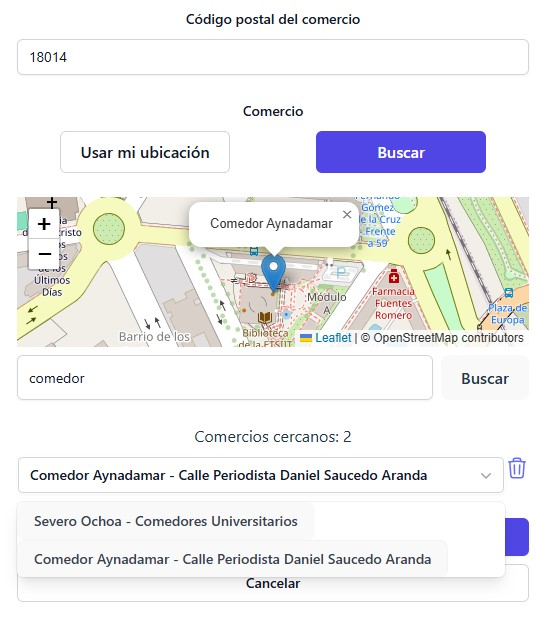
\includegraphics[height = 70mm]{imagenes/mapa_buscador_comercio.jpg}
        \caption{Búsqueda de comercio por buscador en el formulario de gastos}
        \label{fig:mapa_buscador_comercio}
    \end{minipage}\hfill
    \begin{minipage}{0.45\textwidth}
        \centering
        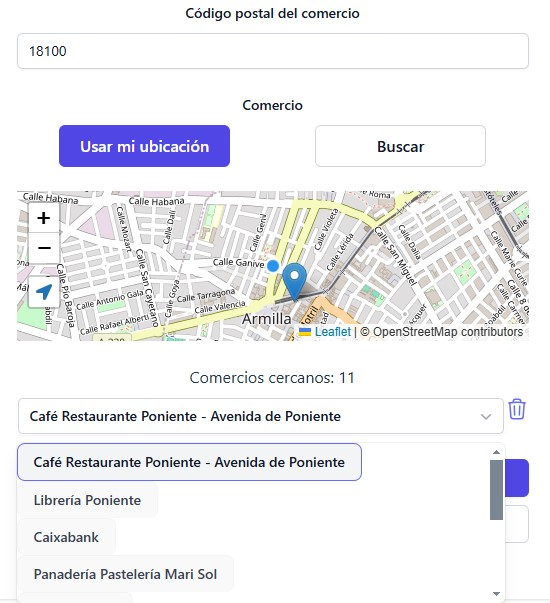
\includegraphics[height = 70mm]{imagenes/mapa_GPS_comercio.jpg}
        \caption{Búsqueda de comercio por geolocalización en el formulario de gastos}
        \label{fig:mapa_GPS_comercio}
    \end{minipage}
\end{figure}

\begin{figure}[ht!]
    \centering
    \begin{minipage}{0.45\textwidth}
        \centering
        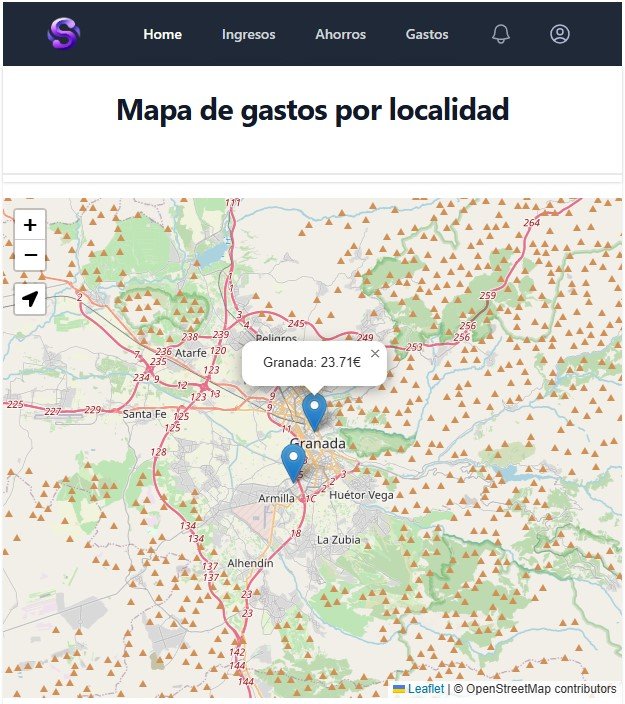
\includegraphics[height = 70mm]{imagenes/mapa_gasto_localidades.jpg}
        \caption{Mapa de gastos por localidad}
        \label{fig:mapa_gasto_localidades}
    \end{minipage}\hfill
    \begin{minipage}{0.45\textwidth}
        \centering
        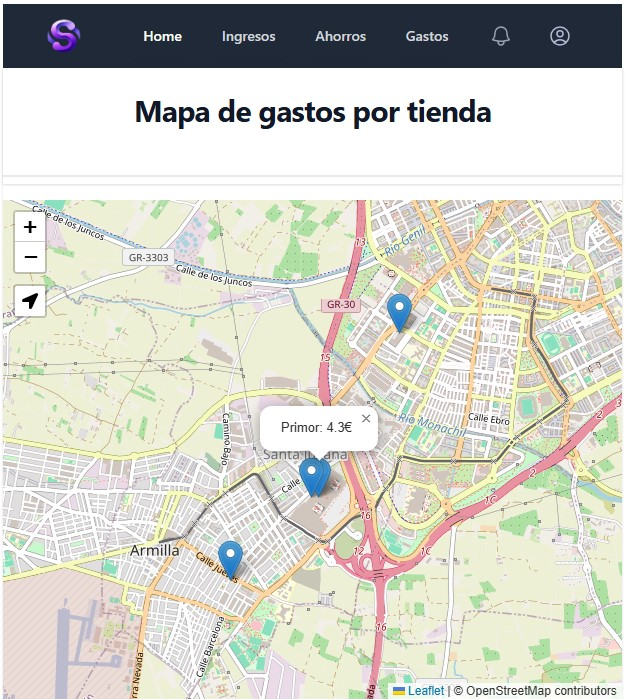
\includegraphics[height = 70mm]{imagenes/mapa_gasto_comercios.jpg}
        \caption{Mapa de gastos por comercio}
        \label{fig:mapa_gasto_comercios}
    \end{minipage}
\end{figure}